\chapter{Knowledge-driven analysis}
\chaptermark{Knowledge-driven analysis}
\label{chap:knowledge}
\graphicspath{{./chapters/5-knowledge/figs/}}

In this chapter we address the problem of understanding comics by automatically improving the consistency of the extracted elements according to the domain knowledge and by inferring new information and launching further processing iteratively.
Detecting these elements and establishing their relationship is crucial towards complete comics understanding.
Using this approach we propose a contribution towards the adaptability of an interpretation system, which corresponds to a hard belt of the literature.
Low level and high level information is used in a complementary and unsupervised way, to progressively identify the different elements of a digitized comic book image and theirs semantic relations.

%We also model the comic book's and the image processing domains knowledge and use an inference engine for information consistency analysis.

%----------------------------------------------
% Introduction
\section{Introduction}
\label{sec:kn:introduction}


Document image analysis is an active field of research which can attain a complete understanding of the semantics of a given document.
One example of the document understanding process is enabling a computer to understand a comic strip story.
In this chapter we propose a knowledge-driven system that can interact with bottom-up and top-down information to progressively understand the content of a document at a semantic level (Figure~\ref{fig:kn:intro_illustration}).

%%%%%%%%%%%%%%%%%%%%%%%%%%%%%%%%%%%%%%%%%%%%%%%%%%%
 \begin{figure}[ht]  %trim=l b r t  width=0.5\textwidth,
   \centering
  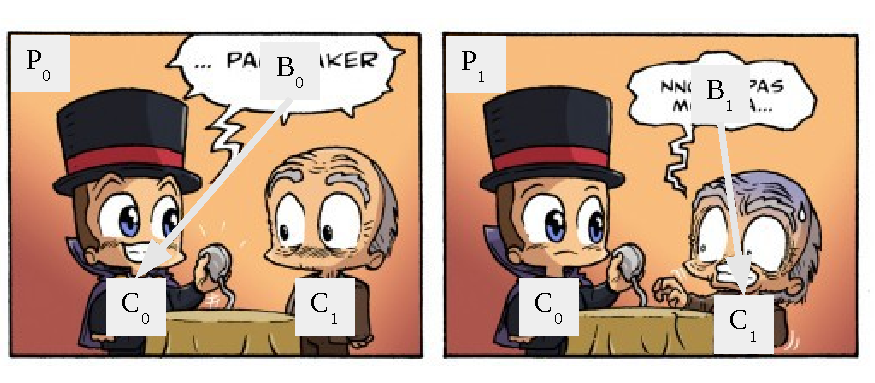
\includegraphics[trim= 0px 10px 3px 10px, clip, width=0.5\textwidth]{intro_illustration.pdf}
  \caption[Example of semantic information understanding]{Example of semantic information understanding. The left panel $P_0$ represents a comics character labelled as $C_0$ saying the content of balloon $B_0$ to another character labelled as $C_1$. In the right panel $P_1$, the character $C_1$ is saying $B_1$ to $C_0$. Image credits:~\cite{Magicien11}. }
  \label{fig:kn:intro_illustration}
 \end{figure}
%%%%%%%%%%%%%%%%%%%%%%%%%%%%%%%%%%%%%%%%%%%%%%%%%%%


The proposed framework is based on interactions between low and high level processing in order to reduce the challenging semantic gap.
The knowledge about low and high level processing is stored in ontologies that are fed by the low level image content extractors.
%Here, the different level of information are given by an image processing and an expert system respectively. 
% We call each image processing algorithm an ``extractor'' of panels, balloons (or bubbles), tails and comic characters (protagonists) according to the type of region they are designed for.
% Low level image content extractors provide a set of regions that feeds a knowledge base.
%in the different extraction processes such as panel and speech balloon improvements and validation (e.g. panel, text, speech balloon) and their combination to guide other feature extractions (e.g. person object).
The knowledge base is associated with properties and constraints that form an ontology.
An expert system uses the ontology to assert the relations between regions and an inference engine to deduct new information in order to perform further image processing.
Note that in the rest of this chapter ``character'' is used in the sense of actor or protagonist of the comics, not as a piece of text.
The main difficulty is to extract but also to model the diversity of styles, format, definition and the differences between design and printing techniques (Figure~\ref{fig:kn:comics_diversity}).

% %%%%%%%%%%%%%%%%%%%%%%%%%%%%%%%%%%%%%%%%%%%%%%%%%%
% \begin{figure}[ht]  %trim=l b r t  width=0.5\textwidth,
%    \centering
%   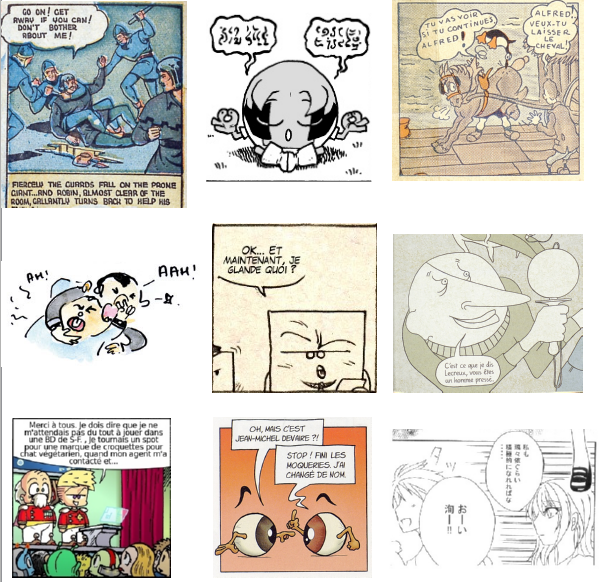
\includegraphics[trim= 4px 0px 0px 0px, clip, width=0.75\textwidth]{comics_diversity.png}
%   \caption{Examples of comic panels that reflect the diversity of comics.}
%   \label{fig:kn:comics_diversity}
%  \end{figure}

% MOVED TO INTRO

% %%%%%%%%%%%%%%%%%%%%%%%%%%%%%%%%%%%%%%%%%%%%%%%%%%


This work is the result of an extensive collaboration with Cl{\'e}ment Gu{\'e}rin, a Ph.D. student working on data mining applied to comic book contents.
All the details about the knowledge models, inference engine and the interactions between the elements can be found in his thesis~\cite{phdthesisGuerin14}.

%--------------------------------------------------
\section{Proposed models} % (fold)
\label{sec:kn:proposed_models}

In this section, we introduce the ontologies developed for automatic analysis and understanding of comic book images.
According to the state of the art review presented Section~\ref{sec:sota:holistic_understanding}, only one previous work proposed an ontology of comics from a philosophical approach~\cite{Aaron2011}.
Cl{\'e}ment Gu{\'e}rin already published some work concerning the inference of the reading order, for panel in the page and balloon in the panel~\cite{Guerin2012Ontologies,phdthesisGuerin14}.
Here we focus on semantic relations within the panel region which is a more recent work in the team.
First, we present a first ontology formalising the concepts related to image processing, data type, the inputs and outputs.
Secondly, we conceptualise the field of comic books oriented to digital image analysis.
Finally, we explain how these ontologies communicate with each other, so they can be used together.

\subsection{Image processing domain} % (fold)
\label{sub:kn:image_processing_domain}

We initially developed a model formalizing the primitive notions of image processing.
This model does not deliberately include any generic concept for comics in order to be used in other areas related to document analysis systems.
It provides support for structuring data from image processing algorithms for subsequent semantic enrichment.
The data produced by such algorithms are generally limited to spatial data, lines, areas, which we will reference under the unique term of \textit{regions of interest} or \textit{ROI} (Region Of Interest) later in this document.
They are defined by their Cartesian coordinates in the orthonormal image from which they are extracted.
From this coarse analysis, we define the first two concepts of our model: \concept{Image} and \concept{ROI}.
Then, a third concept called \concept{Extractor} is create to represent the low level algorithms that are getting the ROI from the image pixels.
Figure~\ref{fig:kn:model_image} shows a visual representation of these concepts altogether.

%%%%%%%%%%%%%%%%%%%%%%%%%%%%%%%%%%%%%%%%%%%%%%%%%%%%%%%%%%%%%%%%%
 \begin{figure}[!ht]
   \centering
  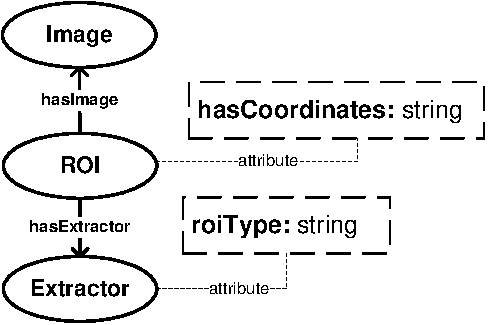
\includegraphics[width=0.5\textwidth]{model_image.pdf}
  \caption[A representation of the image model involved in the expert system]{A representation of the image model involved in the expert system. Concepts are represented by the oval-shaped items; the arrows are the object properties linking them to each other. The dashed rectangles contain the data properties of the concepts they are attached to.}
  \label{fig:kn:model_image}
 \end{figure}
 %%%%%%%%%%%%%%%%%%%%%%%%%%%%%%%%%%%%%%%%%%%%%%%%%%%%%%%%%%%%%%%%%


\paragraph{Image concept} % (fold)
\label{par:image_concept}

The concept of \concept{Image} models the notion of image as a digital object, the input material for image processing systems.
This is the most general concept from which are derived the other concepts of our ontology.
An image processing algorithm works by directly manipulating the pixels of the image, its elementary components.
It can analyse the pixels independently, or grouped in sets of pixels but, in the end, the value and the intensity of each pixel have their importance in the analysis process, and can affect the output results.
Note that for two visually similar images, the individual value of each pixel can vary greatly from one image to another (e.g. high definition, quantization, dithering).
% They may have a different definition (i.e. the size (measured in pixels) different.
% If scanned, if the source documents were the same size images, the difference of definition is the consequence of a difference in scanning resolution.
% The resolution of an image indicates the number of pixels used to discretize an inch of space.
% The higher the resolution, the larger the image is sharp.
Furthermore, the encoding of the visual information in each pixel also varies depending on the image format and the degree of compression applied.
It is important to integrate this information into the model as they define the context of the processing tools.
They greatly help the understanding of the result quality.

\paragraph{Region Of Interest concept} % (fold)
\label{par:region_concept}

% paragraph region_concept (end)
The concept \concept{ROI} derives from the concept \concept{Image} (a region of interest is part of an image).
This concept formalises the notion of region of interest as perceived by the image analysis.
It is composed of connected pixels with visual features corresponding to a certain class of desired visual objects.
The fact that a region of interest is a two-dimensional surface, allows us to represent ROIs as polygons.

% \modif{
% The image model is mostly composed of the concepts of \textit{Image}, \textit{Region of interest (ROI)} and \textit{Extractor}.
% It is based on the fact that the output of image analysis algorithms usually corresponds to spatial regions within the image context.
% A ROI is necessarily extracted from one and only one image, and by one and only one extractor.
% Therefore, the ROI concept is linked to the \textit{Image} and \textit{Extractor} concepts respectively with functional properties \textit{hasImage} and \textit{hasExtractor}.
% %Their coordinates are stored in the OpenGIS Well-Know Text (WKT) format \cite{OpenGISConsortiumInc.2011}.

% Algorithms may have specific characteristics so they don't produce the same set of regions as the result of the analysis of an image.
% Extractors are also usually designed to extract one kind of elements (e.g. panels, balloons and text).
% The purpose of each algorithm is given through the data property \textit{roiType}.
% Figure~\ref{fig:kn:model_image} shows a visual representation of these concepts altogether.
% }

%Moreover, they can be automatic but they also can be manual, if we consider a manual ground truth as a kind of extractor.
%The concept of extractor is extended in two subsumed concepts, \textit{Algorithm} and \textit{GroundTruth}.
%The resulting regions of interest of instances of one of these extractors, are respectively classified as \textit{Automatic regions (ROI\_Auto)} and \textit{Ground truth regions (ROI\_GT)}.

% paragraph image (end)

\paragraph{Region extractor concept} % (fold)
\label{par:region_extractor_concept}

% Une région d'intérêt identifiée par un algorithme de segmentation d'images correspond donc à la proposition par ce dernier d'une zone spatiale de l'image contenant le type d'élément qu'il a été conçu pour détecter.
% Cette région peut effectivement contenir un élément de ce type ou bien contenir tout autre chose.
% La précision de segmentation de l'algorithme est dépendante à la fois des caractéristiques de l'image analysée, de la complexité du domaine d'analyse et bien sûr de la qualité de son implémentation.
% L'ensemble des résultats peut contenir des erreurs.
% Les régions d'intérêt produites ne sont que des propositions demandant à être vérifiées, elles n'ont pas valeur de vérité.\\

% Nous appellerons de tels systèmes de segmentation \textit{extracteurs} dans la suite de ce document.
% La notion d'extracteur est intégrée dans notre modèle sous le concept \concept{Extractor}.
% Relié à celui de \concept{ROI}, il permet d'exprimer le lien étroit entre l'algorithme de traitement d'images et les régions d'intérêt qu'il produit à partir d'une image aux caractéristiques données.
% %de modéliser la connaissance liée aux spécificités d'un extracteur et des régions d'intérêt qu'il produit par rapport à une image aux caractéristiques données.
% Cet ensemble de notions fournit un premier cadre à l'évaluation de la pertinence de l'intégration d'une ROI dans un système plus complet où elle sera amenée à interagir avec d'autres entités.
% Une région d'intérêt provenant d'une image est produite par un et un seul extracteur

A region of interest identified by an algorithm of image segmentation corresponds to the proposal by the latter of a spatial area of the image containing one of the elements that the extractor is designed to detect.
This region can actually contain an element of this type or contain anything else (false alarm).
The accuracy of the segmentation algorithm is dependent on the characteristics of the image, the complexity of the region to extract, the way the parameters are adaptively tuned and of course the quality of its implementation.
% The overall results may contain errors.
Regions of interest are produced only as proposals requesting to be checked.

We call such image analysis systems \textit{Extractors} later in this document.
The notion of extractor is incorporated into our model as \concept{Extractor}.
Linked to the \concept{ROI} concept, it expresses a close connection between the image processing algorithm and the regions of interest that are produced from an image with given characteristics (Figure~\ref{fig:kn:model_image}).
This set of concepts provides an initial framework for the integration of a ROI in a more complete system where it will have to interact with other entities.
A region of interest from an image is produced by a single extractor.

% paragraph paragraph_name (end)

% subsection document_image_processing (end)
\subsection{Comics domain} % (fold)
\label{sub:kn:comics_domain}

We present in this section a conceptualization of the comics domain and its ontological formalisation.
This conceptualisation has been designed by keeping in mind the purpose of use in the context of image analysis.
See Cl{\'e}ment Gu{\'e}rin's thesis for its adaptation to other applications~\cite{phdthesisGuerin14}.
% Amendments may be affixed later in this manuscript in order to make its possible use in other application frameworks.

Comics domain contains two different information levels.
First, the bibliographic information, which are common with any books, about the collection, artist names, International Book Number (ISBN), language, number of page and so on.
Second, the information about all the elements that composes a comic book page (e.g. panel, balloon, text and character), their relations and the corresponding semantic.

\paragraph{Album and pages} % (fold)
\label{par:album_and_pages}

As seen Section~\ref{sec:intro:presentation}, a comic book page is defined as a series of images conveying a message.
These images are spatially juxtaposed in a plane that is called \emph{page} or \emph{board}.
In classical comic strips, a story is told through an ordered succession of pages.
These are represented by the printed pages grouped in an album, which can be from a collection telling a larger story.
The webcomics also make use of pages, materialised by digital images.
In the case of printed comics, a page may extend over one or two pages, rarely more.
A webcomic page is always represented by a single image.

The first two concepts are introduced as \concept{Comic} and \concept{Page}.
These two concepts are related by the property \objProp{hasPage}.
A page is only part of one album.

Bibliographic information of each album are represented by attributes associated to the concept \concept{Comic}.
The album title, the collection (if it exists), its authors, date of publication and ISBN can be given via the corresponding attributes.
The reading direction (left to right or right to left) may be indicated through a Boolean attribute called \dataProp{right2Left}.

%%%%%%%%%%%%%%%%%%%%%%%%%%%%%%%%%%%%%%%%%%%%%%%%%%%%%%%%%%%%%%%
\begin{figure}[h!]
\begin{center}
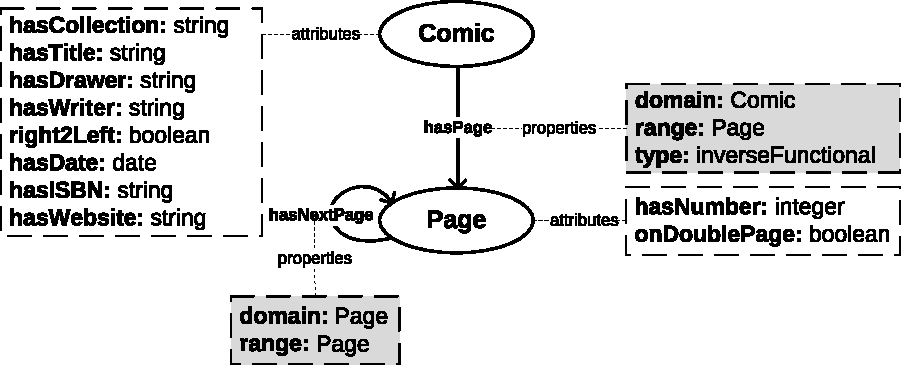
\includegraphics[width=1\textwidth]{model_step1.pdf}
\caption[Initial comics model]{Concepts \concept{Comic} and \concept{Page} with their corresponding relations and attributes.}
\label{fig:model_d_1}
\end{center}
\end{figure}
%%%%%%%%%%%%%%%%%%%%%%%%%%%%%%%%%%%%%%%%%%%%%%%%%%%%%%%%%%%%%%%
% paragraph album_and_pages (end)

\paragraph{Page content} % (fold)
\label{par:page_content}
% Comme présenté dans le chapitre~\ref{chap:codes_bd}, une planche de bande dessinée est le cadre dans lequel sont placées les cases constituant le récit.
% L'ordre de ces cases dans la séquence de lecture est défini par leur position relative les unes par rapport aux autres ainsi que, dans certains cas, l'interprétation personnelle du lecteur.
% L'étude et la génération de la séquence de lecture est l'objet de la section~\ref{sec:ordre}.

We consider that a page consists of panels, which contain drawings such as comic characters and speech balloons.
We initially chose to focus on the relationship between these two types of content.
The consideration of other elements is beyond the scope of this work, although, extracting relevant terms from WordNet might be interesting as well~\cite{Zinger05extracting}.
Balloons contain text lines, embodying the words of the comic characters and the narration of the story.

Panels are represented by the concept \concept{Panel} with the attribute \dataProp{hasRank} which indicates the reading order in the corresponding page.

Balloons or phylacteries, whether they are spoken, thought or narrated, are represented by the concept \concept{Balloon}.
In a similar manner to panels, the balloons must be read in a appropriate order defined by their spatial position in their corresponding panel.
We consider \emph{attached} and not \emph {overlapped} panel because, according to the comic book styles, the balloons are not necessarily spatially positioned within a panel.
Sometimes they are slightly outside or straddle several panels.
Instead, each panel illustrates one action taking place at a fixed time.
Balloons are an integral part of the staging and are attached to a given panel, independently from their relative position to this panel.
Their position in the reading order of a panel is defined by the attribute \dataProp{hasRank} and the property \objProp{hasNextBalloon} binds balloons together.

The balloon tail is represented as the concept \concept{Tail}, and its direction by the attribute \dataProp{hasDirection}.
A balloon may be related to several tails through the property \objProp{hasTail}.

Text lines a designed by the concept \concept{TextLine}.
They are grouped inside balloons with a reading order from top to bottom.
Similarly to panels and balloons concepts, the attribute \dataProp{hasRank} indicates their position in the reading order inside the balloon through the property \objProp{hasNextTextLine}.
Text transcription is stored via the attribute \dataProp{hasText}.


The concepts \concept{Panel}, \concept{Balloon}, \concept{Tail}, \concept{TextLine} and \concept{Character} are disjoint, each element can only be an instance of one of them.  
Figure~\ref{fig:model_d_2} illustrates the addition of these concepts to the ontology.

%%%%%%%%%%%%%%%%%%%%%%%%%%%%%%%%%%%%%%%%%%%%%%%%%%%%%%%%%%%%%%%%%
\begin{figure}[h!]
\begin{center}
%\includegraphics[width=1\textwidth]{img/contributions_domaine/model_step2.pdf}
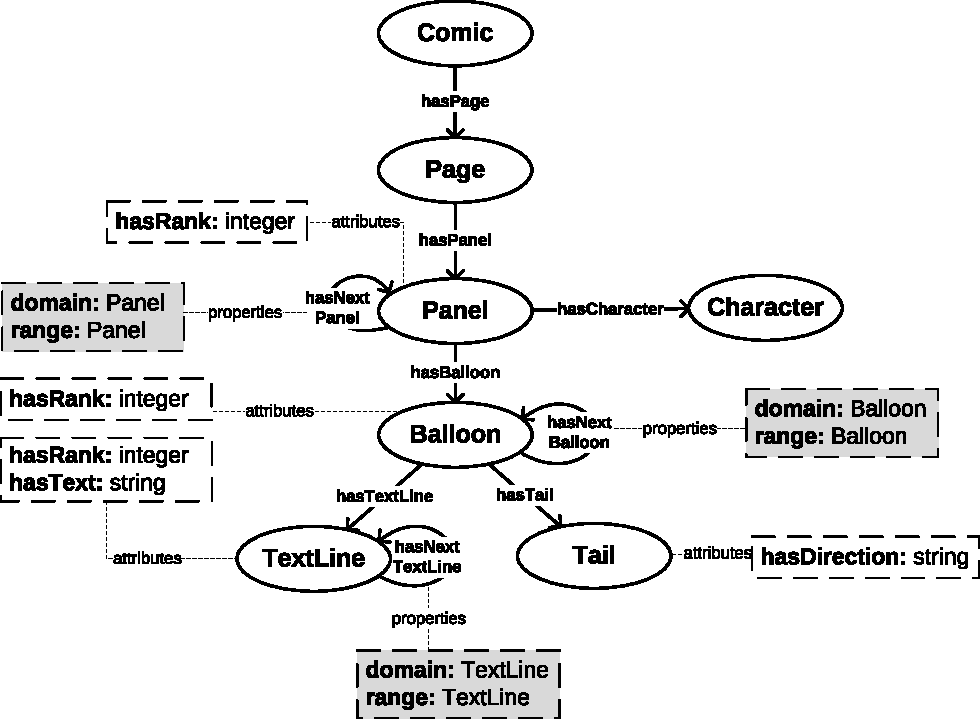
\includegraphics[width=1\textwidth]{model_step2_new.pdf}
\caption[Complete comics model]{Integration of concepts \concept{Panel}, \concept{Balloon}, \concept{Tail}, \concept{TextLine} and \concept{Character} to the initial model Figure~\ref{fig:model_d_1}.}
\label{fig:model_d_2}
\end{center}
\end{figure}
%%%%%%%%%%%%%%%%%%%%%%%%%%%%%%%%%%%%%%%%%%%%%%%%%%%%%%%%%%%%%%%%%

Several properties are introduced into our ontology to represent the links between the various components of a panel.
A panel being relative to the page, the property \objProp{hasPanel} binds an instance of \concept{Page} to an instance of \concept{Panel}.
% The domain and the ranks of the properties ensures that only a page and a panel can be respectively the subject and the object.
% The property \objProp{hasPanel} is also defined functional conversely, a panel that can be part of only one board.

Properties \objProp{hasBalloon} and \objProp{hasCharacter} are formally defined and represent the existing membership between, on one hand, a box and, on the other hand, an instance of \concept{Balloon} and \concept{Character}.
The property \objProp{hasTextLine} represents the link between a text line and a balloon.
% Here we opted for a very constrained conceptualization putting aside some cases significant figure, especially the lines of text scrolls off.
%Cela se justifie dans le cadre d'une analyse automatique d'images, comme nous le présentons au chapitre~\ref{chap:analyseImage}.\\

% Une certaine transitivité dans l'inclusion des éléments les uns par rapport aux autres est observable.
% Les lignes font partie des bulles, faisant elles mêmes, tout comme les personnages, parties des cases.
% Les cases sont regroupées au sein de planches qui, mises les unes à la suite des autres, forment un album.
% L'exploitation de ces appartenances successives trouve un intérêt certain dans un contexte de recherche d'informations au sein d'une base de connaissances.
% Une requête portant sur les albums où apparaissent dans une même case plusieurs personnages prononçant certains termes pourrait par exemple s'affranchir des notions de planche et de bulle.
% paragraph page_content (end)

\paragraph{Specialisation of the content} % (fold)
\label{par:specialisation_of_the_content}

The semantic level of the presented concepts remains at a degree of granularity quite rude, here we present how to refine them.
Balloons might be categorized into two subsets according to their relation to comics character or not.
On one hand the balloons emitted by characters (spoken or thoughts) or elements of the scene (radio, television, etc.), and on the other hand, narrative balloons.
The shape of the speech balloon varies from one author to another.
One feature which seems to be a consensus to discriminate narrative balloons from others, is the presence or not of a tail pointing to the source of the sound.
Concepts \concept{SpeechBalloon} and \concept{NarrativeBalloon} are introduced to represent balloons equipped with a tail or not respectively.
% They are defined by the formulas ~ \ ref {eq: narrativeBalloon} and \ ref {eq: speechBalloon}.

The semantic of text lines in these newly specialised balloons can then be refined accordingly.
Some text lines are carrying elements of speech, while others are for storytelling.
The two corresponding concepts are \concept{SpokenTextLine} and \concept{NarrativeTextLine} respectively.
They are simply defined as text lines belonging to an instance of \concept{SpeechBalloon} or \concept{NarrativeBalloon}.

Speech balloons are usually issued by a character present in the panel.
The link between a character and a speech balloon is expressed through the property \objProp{says}, whose domain \concept{Character} and range \concept{SpeechBalloon}.
The concept \concept{Speaker} represents a character which is emitting a speech balloon.


Figure~\ref{fig:model_d_3} illustrates the relations de introduced for the concepts \concept{Balloon}, \concept{TextLine} et \concept{Character}.

%%%%%%%%%%%%%%%%%%%%%%%%%%%%%%%%%%%%%%%%%%%%%%%%%%%%%%%%%%%%%%%%
\begin{figure}[h!]
\begin{center}
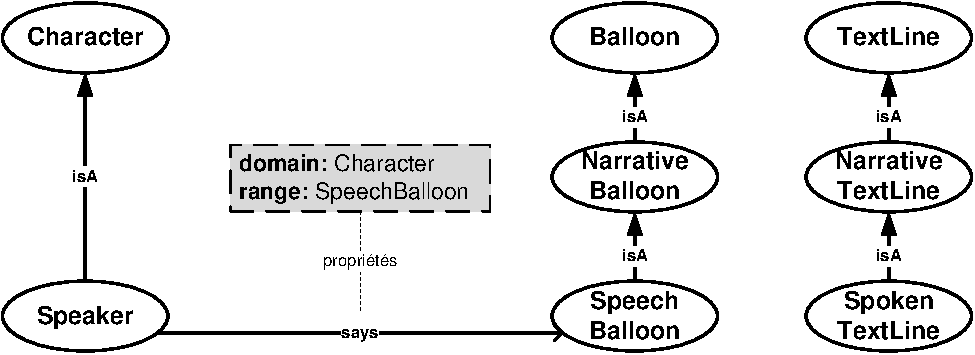
\includegraphics[width=1\textwidth]{model_step2ter_new.pdf}
\caption{Specification of concepts \concept{Character}, \concept{Balloon} and \concept{TextLine}}
\label{fig:model_d_3}
\end{center}
\end{figure}
%%%%%%%%%%%%%%%%%%%%%%%%%%%%%%%%%%%%%%%%%%%%%%%%%%%%%%%%%%%%%%%%

% \modif{TODO: English version}

% Semantic relations were also defined in order to categorise some region types such as balloons into speech balloon $SB$ (versus narrative balloons), characters into speaking characters $SC$ (versus non-speaking characters) and text lines as speech text $ST$ (versus narrative lines):
% \begin{itemize}
%   \item A $SB$ is a balloon $B$ that has a tail and contains text
%   \item A $SC$ is a character $C$ pointed by a tail
%   \item A $ST$ is a text line which is included in one speech balloon
% \end{itemize}

% The term ``pointed'' refers to the fact that the character is included in the part of the panel indicated by the tail. To have a better understanding of how a panel is divided according to tail direction, please refer to Section~\ref{sec:se:tail_to_character}.

% These figures represent the theoretical limit that can be reached with the model in terms of component extraction performance.
% section knowledge_representation (end)

% paragraph specialization_of_the_content (end)

% \modif{TODO: English version}
% The first level of our comics model taxonomy is composed of the concepts of \textit{Album}, \textit{Pages} and \textit{Content}.
% \textit{Album} is linked to \textit{Page} and \textit{Page} to \textit{Content} respectively by the \textit{hasPage} and \textit{hasContent} properties.
% The concept of \textit{Content} stands for any kind of visual element that can appear on an analysed page of comic book.
% It is specialized into the concepts of \textit{Panel}, \textit{Balloon}, \textit{TextLine} and \textit{Character}.
% As it was stated in Section~\ref{sec:kn:constrains_low_level_extraction}, we consider that panels are only contained by a page, characters and balloons by panels and lines of text by balloons.
% This is modelled with object properties with constrained domain and range.
% The \textit{hasPanel}, \textit{hasBalloon}, \textit{hasTextLine} and \textit{hasCharacter} properties link a page to a panel, a panel to a balloon, a balloon to a line and a panel to a character, respectively.

% Even if that does not cover every situation (text lines can sometimes be found outside of balloons, e.g onomatopoeia), these constrained properties are necessary to use these models as validation tools.
% %While we know that it does not cover every different kind of comics material, it is necessary if we want it constrained enough to be usable as a segmentation validation tool.
% The concepts of \textit{Speaker}, \textit{SpeechBalloon} and \textit{SpokenTextLine} are subsumed by \textit{Character}, \textit{Balloon} and \textit{TextLine} respectively and are derived with an OWL translation of the rules defined Section~\ref{sec:kn:constrains_low_level_extraction}.
% This hierarchy is visually represented in Figure~\ref{fig:kn:model_image}.
% Balloons and text lines are also enriched by some attributes, like the direction indicated by the tail (\textit{tailDirection}) or the textual transcription of the text lines (\textit{hasText}).

 % \begin{figure}[!ht]
 %   \centering
 %  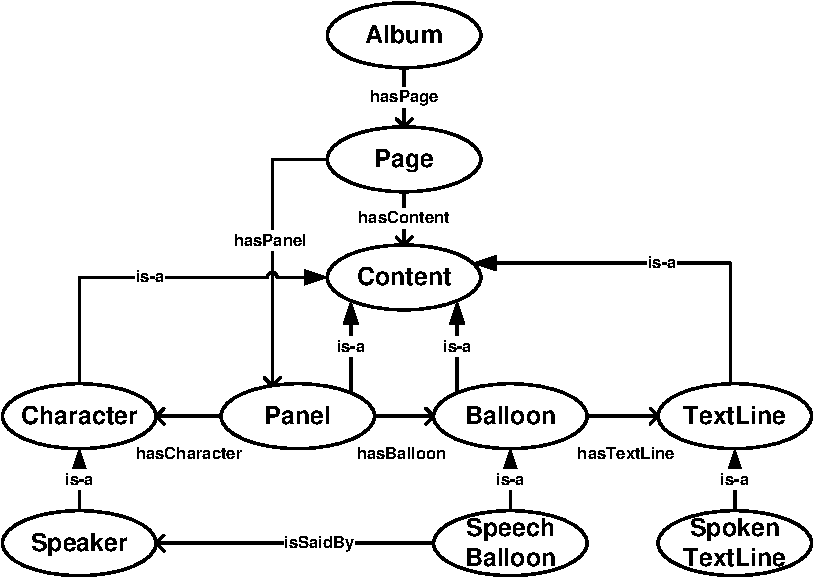
\includegraphics[width=0.7\textwidth]{model_comics.pdf}
 %  \caption[A representation of the main aspects of the comics model involved in the expert system]{A representation of the main aspects of the comics model involved in the expert system. Concepts are represented by the oval-shaped items, full arrows represent subsumption relations, simple arrows are the object properties linking them to each others. Attributes are not displayed to make it more comprehensible.}
 %  \label{fig:kn:model_image}
 % \end{figure}

% subsection comics_domain (end)

\subsection{Model interactions} % (fold)
\label{sub:model_interactions}

In this section we present the interactions between the image and comics ontologies so that they can communicate and combine their reasoning capabilities.
We call $\mathcal{O}_{image}$ and $\mathcal{O}_{comics}$ the ontologies of image and comics respectively presented Sections~\ref{sub:kn:image_processing_domain} and \ref{sub:kn:comics_domain}.
% Both models have been developed for comics image analysis.
% In this context, we consider that the scanned image is the raw material supplied to an algorithm so that it can extract its contents.

% Comme cela a été souligné précédemment, un algorithme d'analyse d'images a pour objectif la détection de caractéristiques visuelles discriminant un type d'objet particulier.
% Dans notre cas, les extracteurs développés concernent les cases, les bulles, 
% la queue des bulles, 
% le texte et les personnages.

Figure~\ref{fig:kn:interactions} illustrates the interactions between the ontologies.

%%%%%%%%%%%%%%%%%%%%%%%%%%%%%%%%%%%%%%%%%%%%%%%%%%%%%%%%%%%%%%%%%%%%%%%%%
\begin{figure}[h!]
\begin{center}
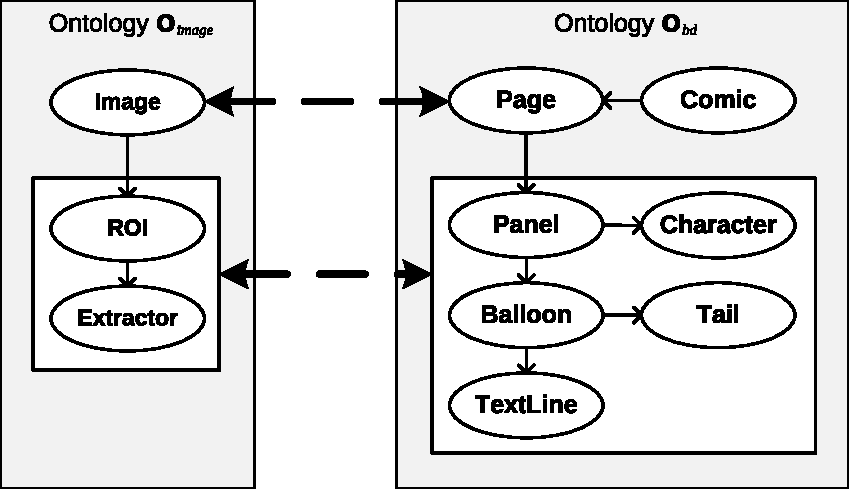
\includegraphics[width=0.8\textwidth]{interactions.pdf}
\caption{Interaction between the two ontologies.}
\label{fig:kn:interactions}
\end{center}
\end{figure}
%%%%%%%%%%%%%%%%%%%%%%%%%%%%%%%%%%%%%%%%%%%%%%%%%%%%%%%%%%%%%%%%%%%%%%%%%

The image and comics models are linked through two bridges.
First, the \concept{Image} concept from $\mathcal{O}_{image}$ and the \concept{Page} concept from $\mathcal{O}_{comics}$ are made equivalent.
This ensures that all extracted content related to an image are equally related to a corresponding page in the comics domain $Page \equiv  Image$.

Second, the classes $Cl=\{Panel$, $Balloon$, $Tail$, $TextLine$, $Character\}$ are defined as equivalent to the corresponding set of regions of interest $roiType = \{panels$, $balloons$, $tail$, $text lines$, $characters\}$ (Equation~\ref{eq:kn:class_region_equivalence}).% that have an extractor which purpose is to extract the corresponding panels (resp. balloons, text lines and characters).
  

\begin{equation}
\label{eq:kn:class_region_equivalence}
\begin{split}
Cl_i  \equiv \text{ROI} \textbf{ and } (hasExtractor \textbf{ some } (roiType \textbf{ value } Sr_i ))
\end{split}
\end{equation}

% subsection model_interactions (end)

% section proposed_models (end)

%--------------------------------------------------
\section{Expert system for contextual analysis} % (fold)
\label{sec:kn:expert_system}

In this section we refer to the algorithmic part related to image processing as \emph{low level} processing. 
The proposed system composed by the developed ontologies and an inference engine (\emph{high level} processing) is called \emph{expert system} for clarity.
A dynamic communication is maintained between low and high level processing of the overall analysis system, this section will detail its operation.


\subsection{Interactions between low and high level processing} % (fold)
\label{sub:interactions_between_low_and_high_level_processing}


We consider the ontologies $\mathcal{O}_{image}$ and $\mathcal{O}_{comics}$ developed as integral parts of an expert system that provides an interpretation framework for low level image content.
The purpose of the expert system is to interact with the low level iteratively in order to progressively understand the content of an image, moving from simple to more complex elements.
This approach is similar to~\cite{Sciascio2011Structured} except that in our case the definition of the complex object is not a composition of simple objects but context-driven.

The expert system, represented by the diagram in Figure~\ref{fig:kn:generic_expert_system}, includes both ontologies forming our knowledge base.
This knowledge base, once populated by data from the low-level system, is queried by an inference engine (e.g. Racer~\cite{Haarslev2012}] or Pellet~\cite{Sirin2007a}) to extract logical conclusions, depending on the data and their consistency compared to the formalised knowledge.

These logical conclusions may include a validation of extracted elements, rejection or creation of elements referred to the image processing system.


%%%%%%%%%%%%%%%%%%%%%%%%%%%%%%%%%%%%%%%%%%%%%%%%%%%
 \begin{figure}[!ht]  %trim=l b r t  width=0.5\textwidth,
   \centering
  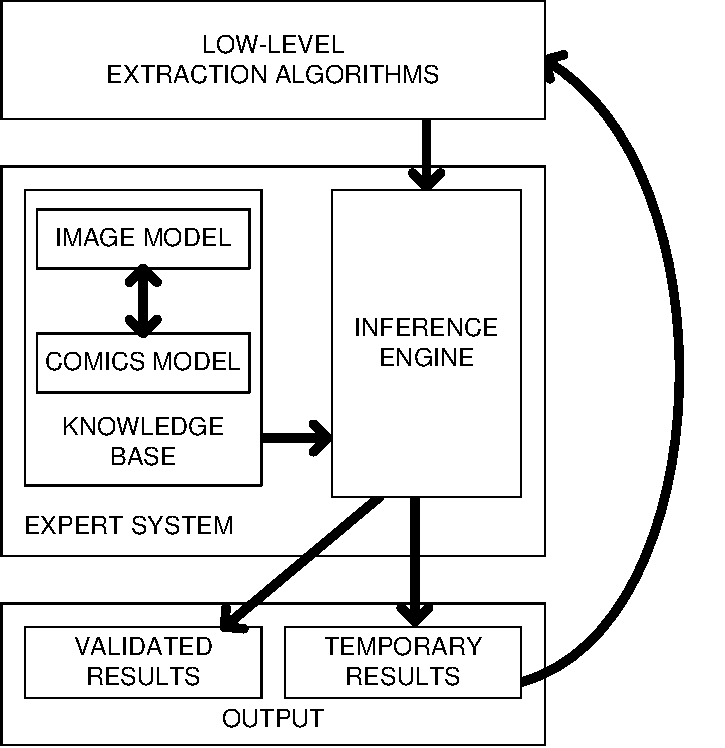
\includegraphics[trim= 0px 0px 0px 0px, clip, width=0.5\textwidth]{expert_system.pdf}
  \caption[Generic representation of the expert system and the relationship between knowledge base, the inference engine and the low-level algorithms]{Generic representation of the expert system and the relationship between knowledge base, the inference engine and the low-level algorithms.}
  \label{fig:kn:generic_expert_system}
 \end{figure}
%%%%%%%%%%%%%%%%%%%%%%%%%%%%%%%%%%%%%%%%%%%%%%%%%%%

%This knowledge can be represented by all the relations between the elements that constitute a document from this collection.
The low level algorithms have been designed to extract specific information from the whole image or a specific region.
Low and high level systems interact in a loop to feed the knowledge base until there is a complete and consistent understanding of the document, according to the knowledge domain. 
Figure~\ref{fig:kn:process_loop} illustrates this loop interacting between the two level of information.

%%%%%%%%%%%%%%%%%%%%%%%%%%%%%%%%%%%%%%%%%%%%%%%%%%%
 \begin{figure}[!ht]  %trim=l b r t  width=0.5\textwidth,
   \centering
  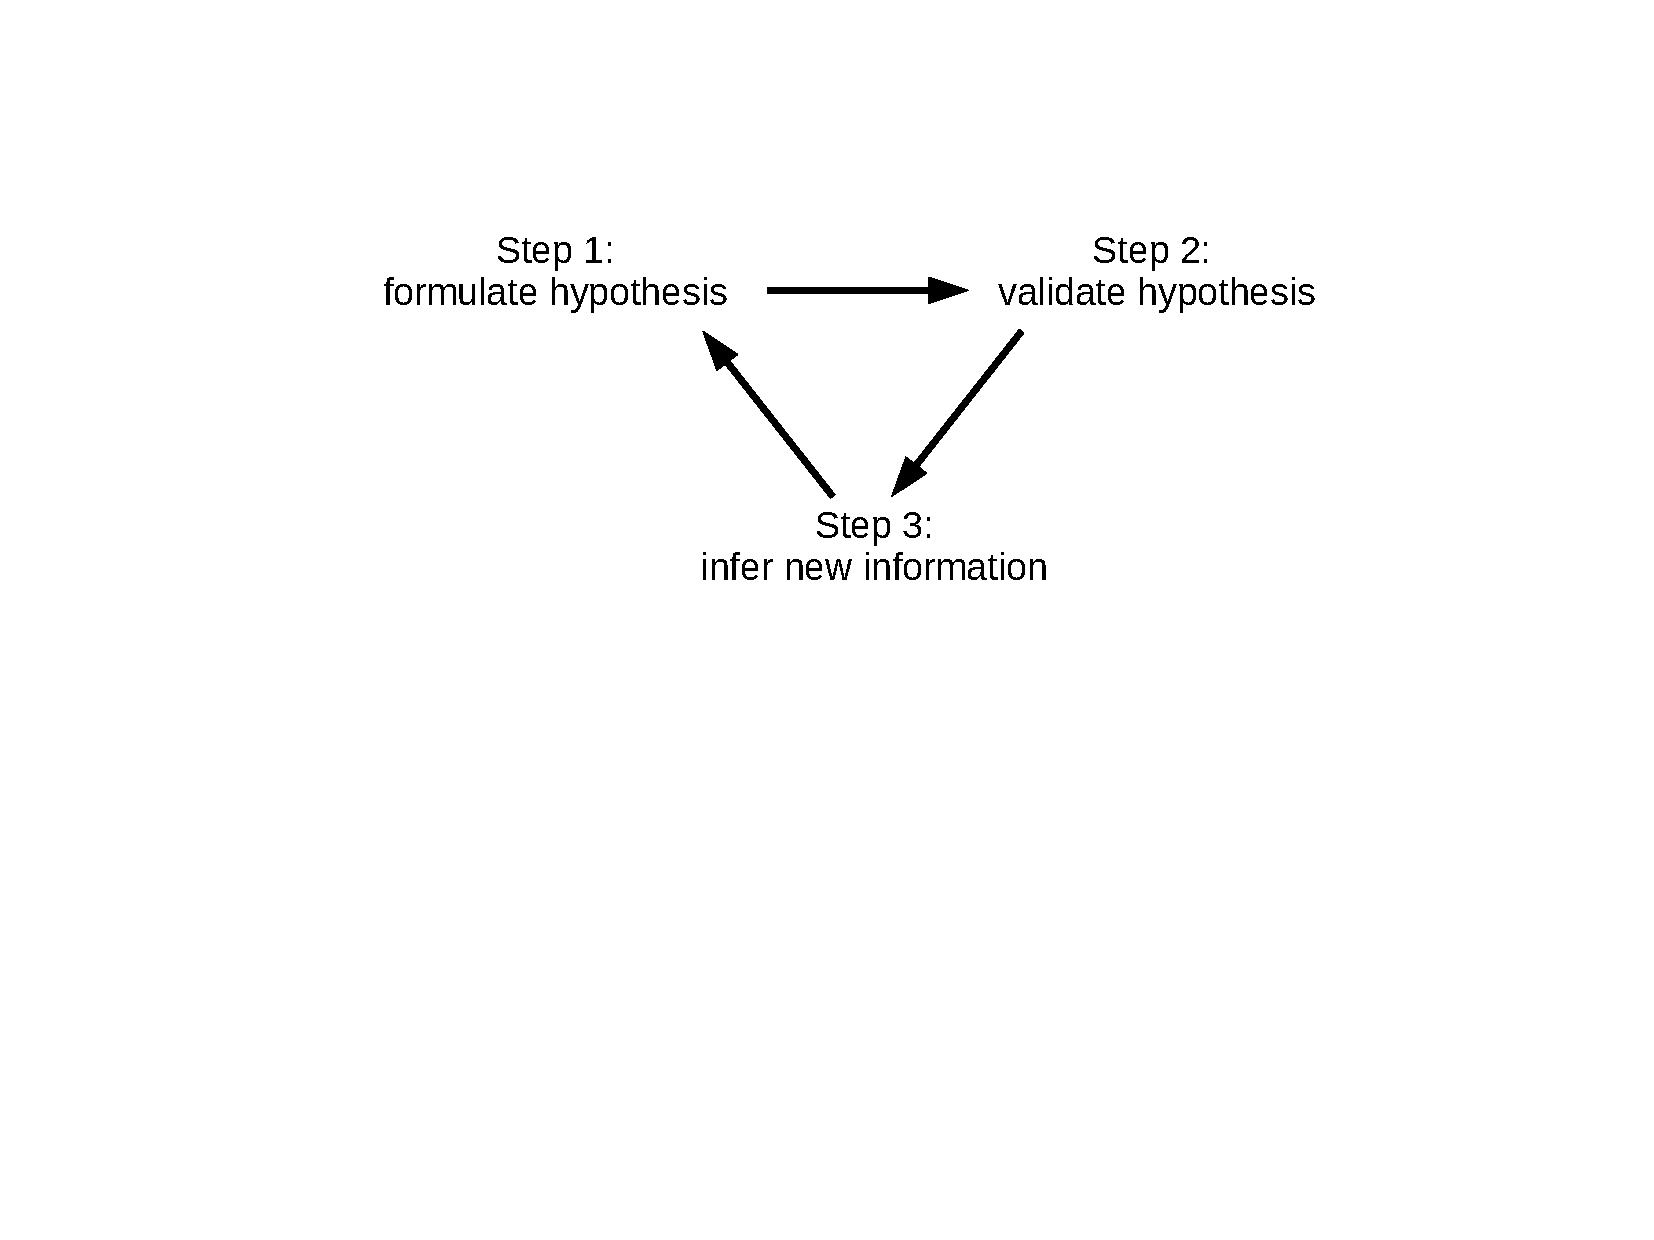
\includegraphics[trim= 140px 315px 100px 95px, clip, width=0.7\textwidth]{process_loop.pdf}
  \caption[Process loop of the knowledge-driven system]{Process loop of the framework.}
  \label{fig:kn:process_loop}
 \end{figure}
%%%%%%%%%%%%%%%%%%%%%%%%%%%%%%%%%%%%%%%%%%%%%%%%%%%

% In Figure~\ref{fig:kn:process_loop}, the starting point is step 1 (formulate hypothesis) where low level processing give basic information to the expert system (populating).
% %, preferably with a high recall.
% Then, step 2 (validate hypothesis) assesses the valid elements and removes obvious mistakes, and in step 3 we infer new information based on the previous information and the knowledge base.
% In the next iteration of the process loop, the newly validated information can be used by low level processing (e.g. new parameters, region of interest) to extract more complex elements from the image and so on.
% This loop can be run as many times as new information is discovered (until being idempotent).

In step 1, the low level system propose to the expert system assumptions about a first set of segmented regions in the image.
These regions are labelled according to their supposed type according to the extractor (panel, balloon, text, etc.).
In the second step, the expert system evaluates these assumptions, validates correct ones and deletes others.
Note the deletion is the simplest action we can perform from invalid information but we are currently investigating other scenarios such as switching or changing element labels.
In the third step, new information is inferred from valid assumptions, put in perspective of the domain knowledge.
These are referred to the corresponding low level extractor that will use them, during the following iteration, to extract more complex elements such as the comic characters.
This loop can be run as many times as new information is discovered.


% In our system, the expert system includes two models, one formalizing the raw data from algorithms (\emph{Image model}) and the other modelling the domain knowledge of the comic books (\emph{Comics model}).
% These two models are ontologies that work together to
%This knowledge is formalized in an ontology that 
% express the relations between the primary elements of a document that can be considered as being stable through all instances of the studied domain (Figure~\ref{fig:kn:generic_expert_system}).
% Thus, the expression of the constraints applied both to the elements and their relations have to be specific enough because these constraints will be considered as the reference knowledge for the detection of potential errors of the low-level extraction algorithm output.


% subsection interactions_between_low_and_high_level_processing (end)


% section expert_system (end)

\subsection{Constraints for the low level extractions} % (fold)
\label{sec:kn:constrains_low_level_extraction}

In our model, knowledge is modelled though the categorization of each element composing a page, combined with a set of topological relation with these elements.
In our context, the elements that compose a given image $I$ are panels $P$, balloons $B$, tails $Q$, text $T$ and characters $C$, as well as the set of topological and semantic relations between them.
Because comics, as an art form, do not follow any strict specifications it is really hard to build a perfect model which is valid for all kinds of comics.
There are some instances of comic books without balloons or without panels.
If webcomics are also considered, then a comic is not even necessarily composed of pages.
A model that would be true for every type of comic book would be too general to be of any use in this work.
Instead we define a general comic book model with more constrained properties that represent a large subset of comics (Franco-Belgian, Japanese and American).
The main advantage is that it can be adapted to any kind of document images by defining properties according to the application domain.
We define the general properties of comics as follows:

\begin{itemize}
  \item A panel $P$ is related to one and only one comics page
  \item A balloon $B$ is related to one and only one panel
  \item A character $C$ is related to one and only one panel
  % \item A same character can appear only once in a panel
  \item A text line $T$ is related to one and only one balloon $B$
\end{itemize}

Despite the fact that authors are free in their layout choices, they follow general use conventions widely adopted by comic book's authors in order to avoid confusing the reader~\cite{Laine2010,duc1997art}.
The depicted elements and their place in the page must be clearly identifiable at first sight, meaning, for instance, that text is contained by the balloons which are included inside panels just like the characters.
Whereas one can find some instances of balloons breaking out of their panel, these are usually kept to a minimum.

Therefore, the term ``related'' refers to the situation where an object is overlapped (a fortiori, contained) by another over a \emph{significant} proportion of its surface.
In the case of multiple intersections, only the smallest container is considered.
When the element is fully contained in several other items, the smallest container is consequently the direct container (e.g. a text line must be considered as being included inside a balloon before being included inside the panel containing that balloon).

\section{Processing sequence} % (fold)
\label{sec:kn:processing_sequence}

The expert system asserts the extraction of simple elements such as panels, text, balloons and tails in order to infer speech balloons before searching for more complex elements (e.g. comic book characters) based on the context defined by the simple elements and their relations.
This can be demonstrated with the first two iterations of the process loop (Figure~\ref{fig:kn:process_loop}).

The first iteration treats simple elements such as panels, balloons and text lines.
They are called simple because they have a relatively regular structure.
% and have already received the attention of numerous works in the past.
During the second iteration of the process loop, the detection of the comic characters, more complex in their visual diversity is discussed.

The different stages of the process are illustrated through the couple of panels presented in Figure~\ref{fig:casesExampleReconnaissance}.

%%%%%%%%%%%%%%%%%%%%%%%%%%%%%%%%%%%%%%%%%%%%%%%%%%%%%%%%%%%%%%%%%%%%%%%%%%%%%
\begin{figure}[!h]  %trim=l b r t  width=0.5\textwidth,
\centering
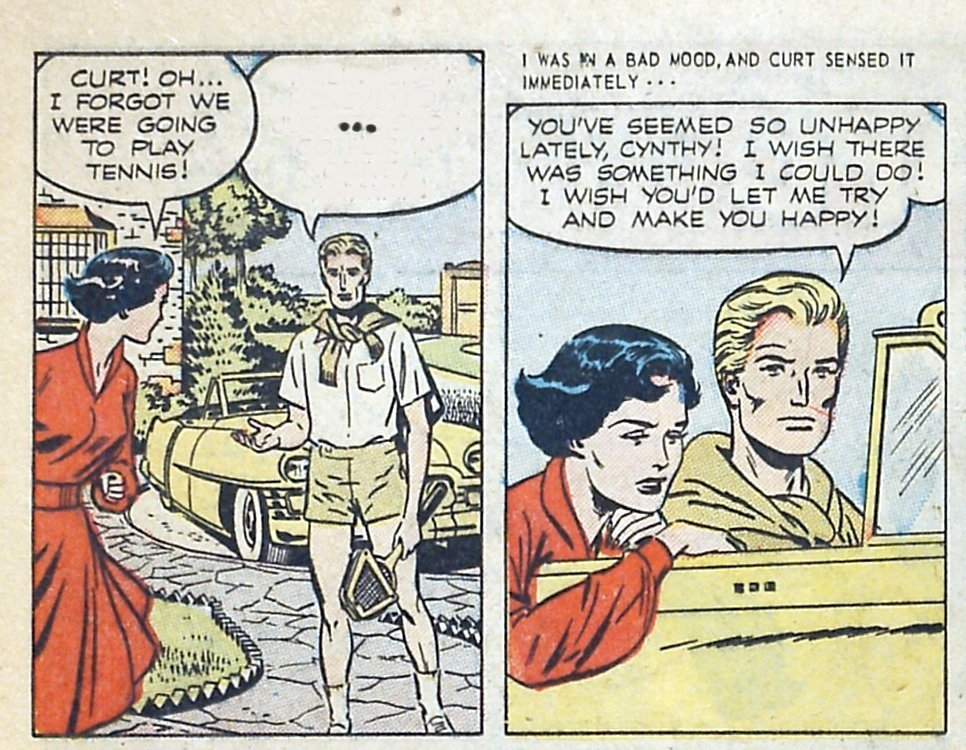
\includegraphics[width=0.5\textwidth]{process_illustration.jpg}
\caption[Original panels used to illustrate the different stages of the processing sequence]{Original panels used to illustrate the different stages of the processing sequence. Image credits:~\cite{Jay53}.}
\label{fig:casesExampleReconnaissance}
\end{figure}
%%%%%%%%%%%%%%%%%%%%%%%%%%%%%%%%%%%%%%%%%%%%%%%%%%%%%%%%%%%%%%%%%%%%%%%%%%%%%

\subsection{Simple element extraction} % (fold)
\label{sub:simple_element_extraction}

\paragraph{Iteration 1 - step 1 (hypothesis)} % (fold)
\label{par:step_1}
The initial extraction of panels, text and balloons feeds the knowledge base.
All the elements are extracted independently using the method proposed Chapter~\ref{chap:independent}.
All these elements are assumptions to be validated by the expert system.
In Figure~\ref{fig:kn:graph0}, dashed elements represent the initial hypotheses and each colour a result from a different extractor.
Note that extraction errors can take place at this stage and that these errors can be recovered by the system at a later stage.
% have been introduced in the example in order to demonstrate how the proposed system can recover them.
% The regions that have been validated by the expert system have a solid border, others a dashed border.


%%%%%%%%%%%%%%%%%%%%%%%%%%%%%%%%%%%%%%%%%%%%%%%%%%%
\begin{figure}[h!] %trim=l b r t  width=0.5\textwidth,
\begin{center}
\subfloat[]{\label{fig:kn:process_illustration_hypo_1}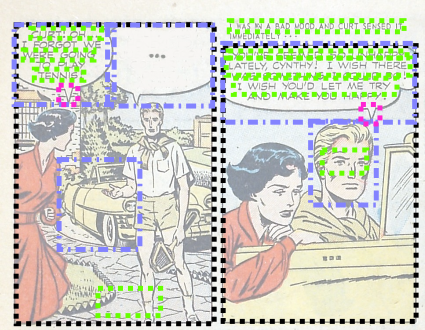
\includegraphics[width=0.4\textwidth]{process_illustration_hypo_1.png}} \hspace{0.5em}
%\subfloat[]{\label{fig:kn:process_illustration_hypo_1}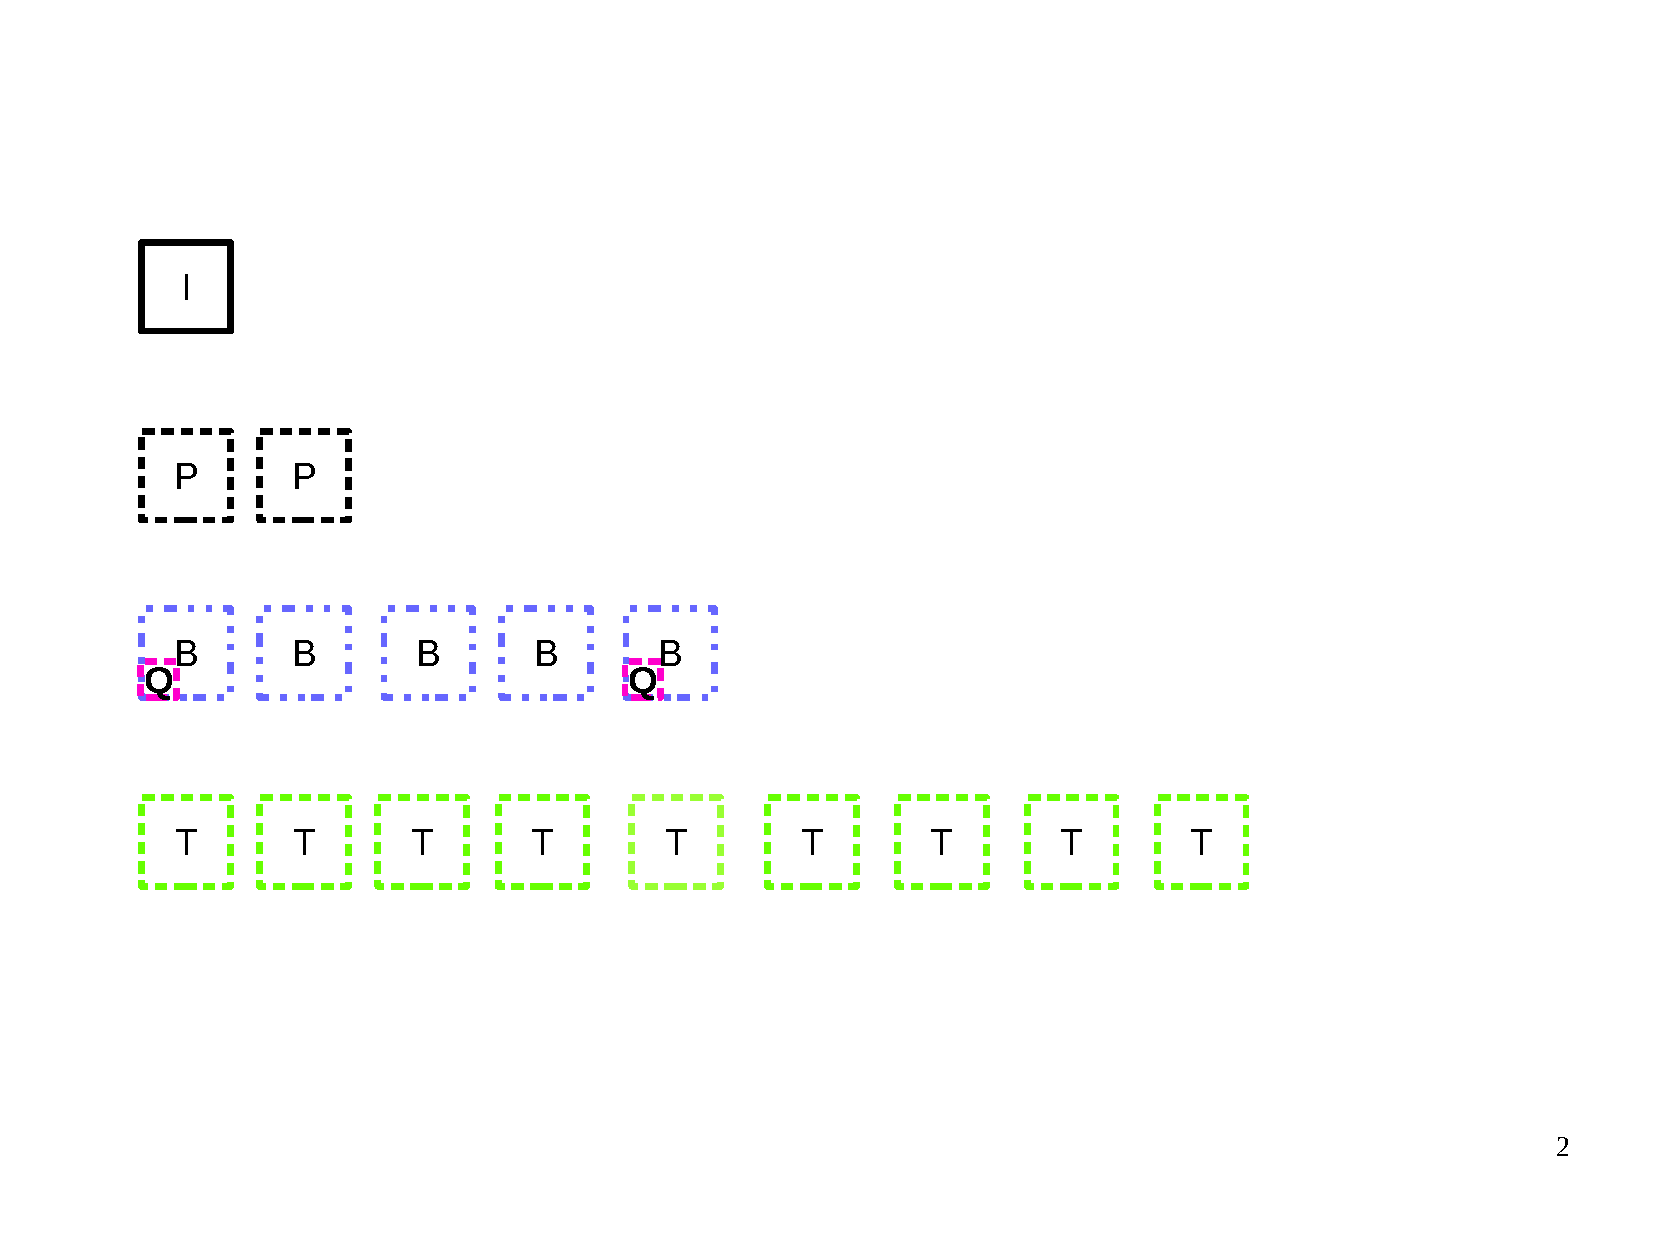
\includegraphics[trim= 65px 168px 150px 110px, clip, width=0.55\textwidth]{graph_init_1_non_orderred.pdf}}
\subfloat[]{\label{fig:kn:process_illustration_hypo_1}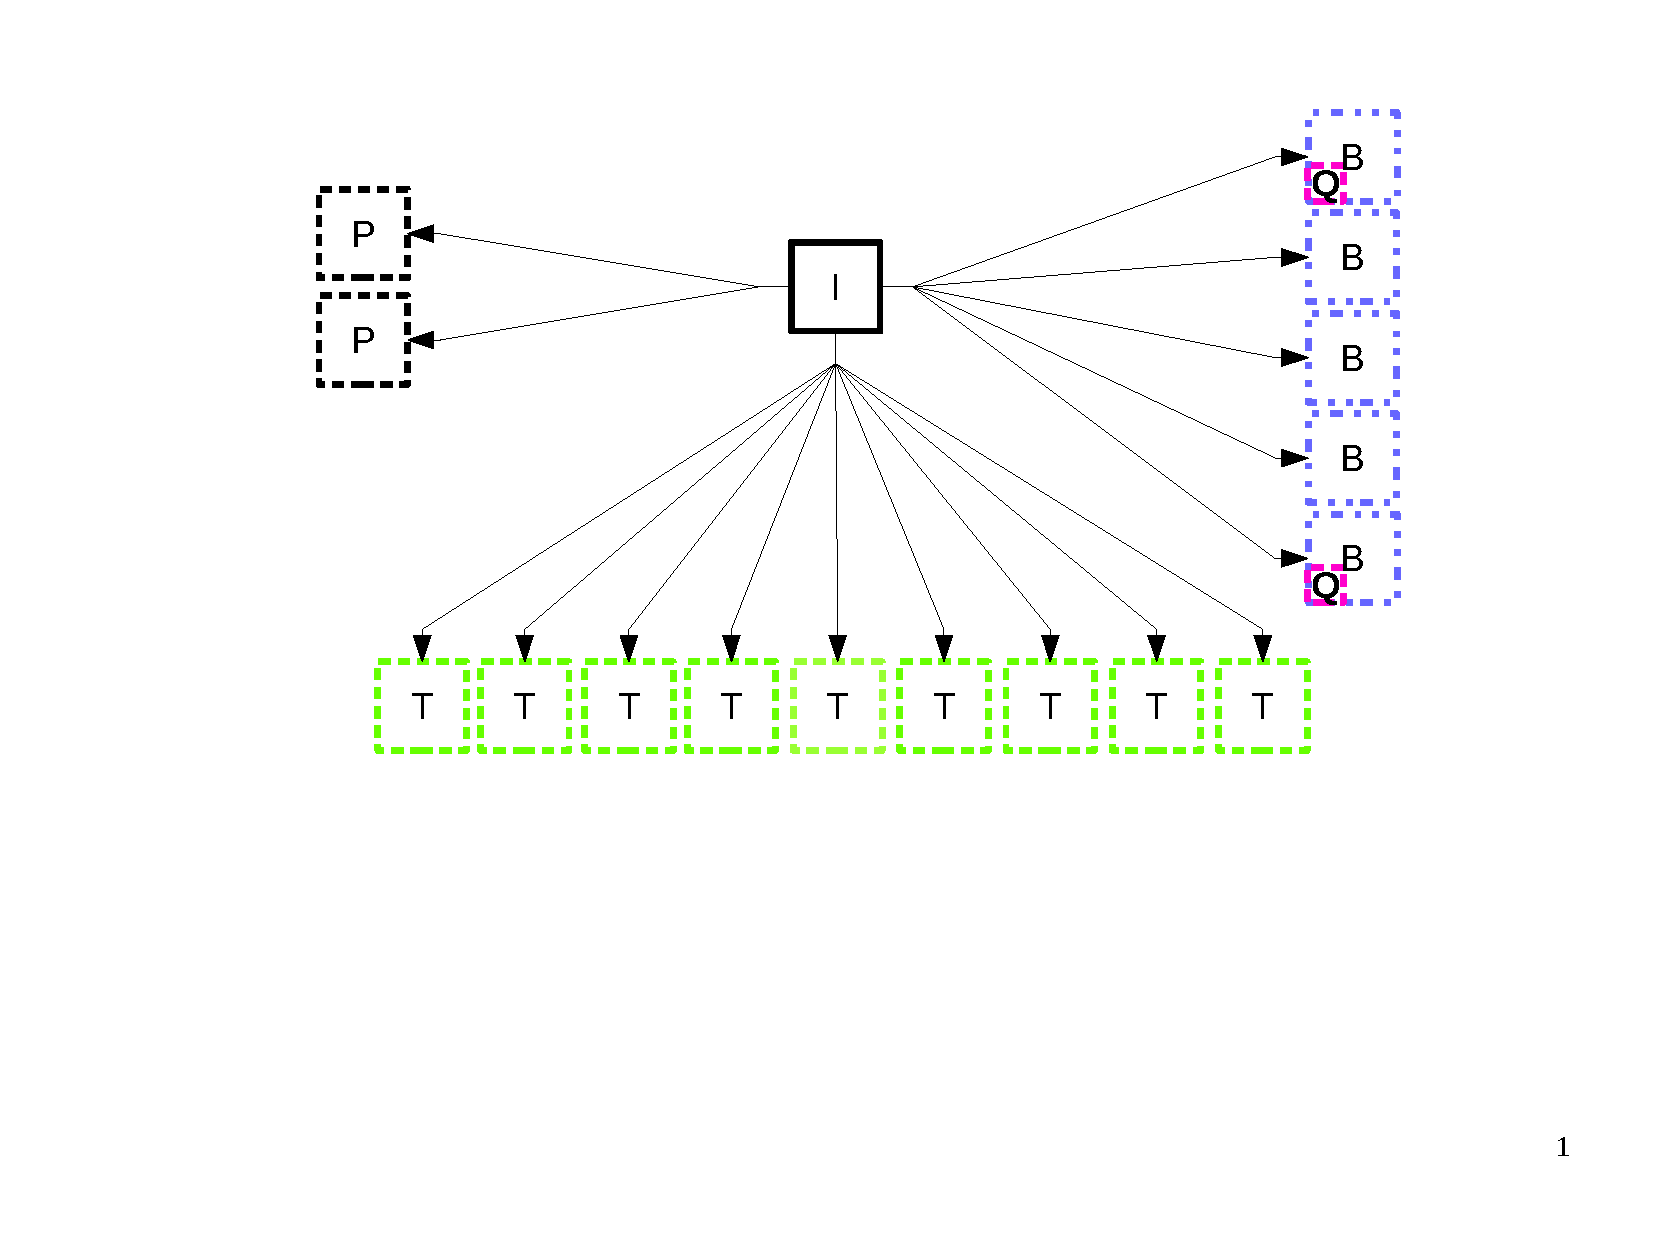
\includegraphics[trim= 150px 230px 100px 40px, clip, width=0.55\textwidth]{graph_init_1bis.pdf}}
\caption[Initial hypothesis about the content of a given image]{Initial hypothesis (dashed elements) about the content of a given image $I$ after the initial extractions of panels $P$, text $T$ and balloons $B$ with tails $Q$.
}
\label{fig:kn:graph0}
\end{center}
\end{figure}

 % \begin{figure}[!ht]  %trim=l b r t  width=0.5\textwidth,
 %   \centering
 %   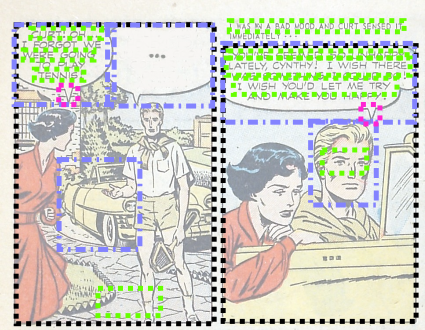
\includegraphics[trim= 0px 0px 0px 0px, clip, width=0.5\textwidth]{process_illustration_hypo_1.png}\\
 %  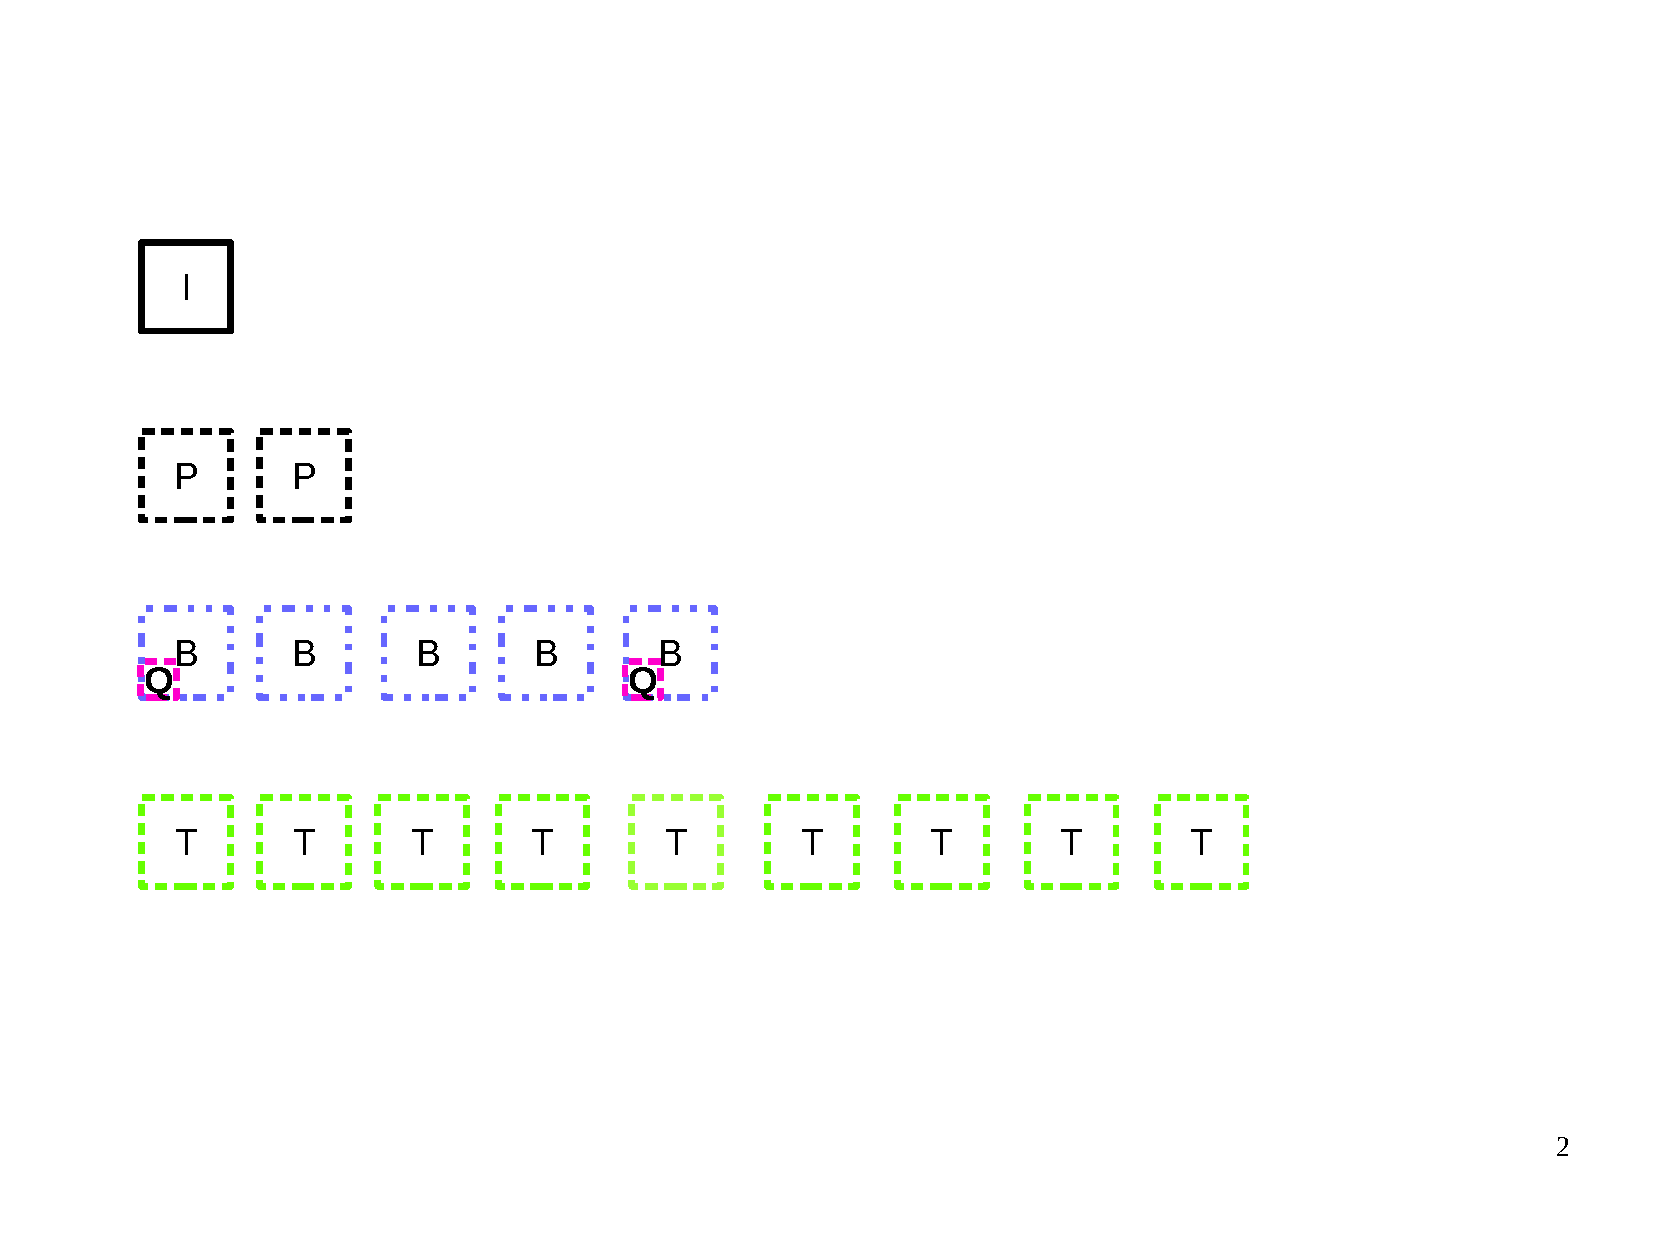
\includegraphics[trim= 30px 168px 100px 110px, clip, width=0.8\textwidth]{graph_init_1_non_orderred.pdf}
 %  \caption[Initial hypothesis about the content of a given image]{Initial hypothesis (dashed elements) about the content of a given image $I$ after the initial extractions of panels $P$, text $T$ and balloons $B$ with tails $Q$.
 %  }
 %  \label{fig:kn:graph0}
 % \end{figure}
%%%%%%%%%%%%%%%%%%%%%%%%%%%%%%%%%%%%%%%%%%%%%%%%%%%

\paragraph{Iteration 1 - step 2 (validation)} % (fold)
\label{par:step_2}
At the second step, the hypotheses proposed by the low level system are compared to the constraints formalized in the ontology.
The extracted regions are first categorized as panels, balloons and text lines thanks to the rules presented in Section~\ref{sub:model_interactions}, interpreted by the inference engine.
Then each element $e$ is linked to its direct container $E$.
This is selected from the set of extracted regions as described in Section~\ref{sec:kn:constrains_low_level_extraction}.
If the system is unable to find a container for an element $e$ from the set of extracted regions, the page is then considered as the container of $e$.

In order to validate the assumption of all the elements in $E$, they are simply considered as instances of the concept $\concept{ROI}_i$.
We voluntarily do not take into account of their class in the ontology $\mathcal{O}_ {bd}$.
This has for effect to introduce inconsistencies between the type of container and the domain of a property resulting from \objProp{hasContent}, making the model inconsistent.
These inconsistencies allow to highlighting possible errors made during the low-level processing.
The inference engine is stated again on the ontology and inconsistencies are treated one after the other.

In this work, we focused on optimizing the reliability of the results.
% We have chosen to focus on the accuracy of extractions rather than completeness.
% Detection of misclassification, such as a box has been segmented by the extractor of bubbles, and the prominence of items that may have been forgotten are both short-term prospects of this work.
% Currently, our system is able to handle the following reasons for inconsistency:
We have chosen to focus on increasing the extraction precision rather than completeness by deleting the elements that did not fit the proposed model.
The detection of misclassified elements (e.g panel actually being a balloon) and the proposition of missed elements (e.g. a missed balloon around a group of text lines) are both short term perspectives of this work.
For the time being, our system can handle, without being limited to, the following inconsistencies:

\begin{itemize}
  \item \textbf{A page (p) contains a balloon (b), a text line (t)}: b or t is deleted.
  \item \textbf{A panel (p1) contains a panel (p2) or a text line (t)}: p2 or t is deleted.
  \item \textbf{A balloon (b) contains a panel (p)}: if p contains some balloons and b does not contain any text lines, b is deleted, otherwise, p is deleted.
  \item \textbf{A balloon (b1) contains a balloon (b2)}: if b1 does not contain any line then b1 is deleted, otherwise b2 is deleted.
  % \item \textbf{A balloon (b) contains a character (c)}: c is deleted.
  \item \textbf{A text line (t) contains a panel (p)}: if p does not contain any balloon then p is deleted, otherwise t is deleted.
  \item \textbf{A text line (t) contains a balloon (b)}: if b does not contain any text line then b is deleted, otherwise t is deleted.
  \item \textbf{A text line (t1) contains a text line (t2)}: if t1 contains other lines then t1 is deleted, otherwise t2 is deleted.
  % \item \textbf{A text line (t) contains a character (c)}: c is deleted.
  % \item \textbf{A character (c) contains a panel (p), a balloon (b) or a text line (t)}: c is deleted.  
  % \item \textbf{A character (c1) contains a character (c2)}: c2 is deleted.
\end{itemize}

The term ``related'' refers to the relation of membership of an element to another, as described in Section~\ref{sec:kn:constrains_low_level_extraction}.
Figure~\ref{fig:kn:graph_valid_initial} illustrates the current organisation of the extracted elements.
They have been structured according to the model definition Section~\ref{sub:kn:comics_domain}.
Validated elements are illustrated in solid lines while other still dashed.


%%%%%%%%%%%%%%%%%%%%%%%%%%%%%%%%%%%%%%%%%%%%%%%%%%%
 \begin{figure}[!ht]  %trim=l b r t  width=0.5\textwidth,
   \center
   \subfloat[]{\label{fig:kn:process_illustration_valid_1}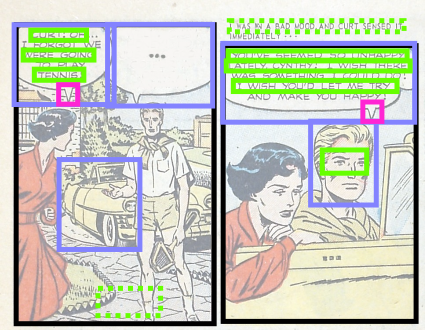
\includegraphics[width=0.4\textwidth]{process_illustration_valid_1.png}} \hspace{0.5em}
   \subfloat[]{\label{fig:kn:graph_valid_1}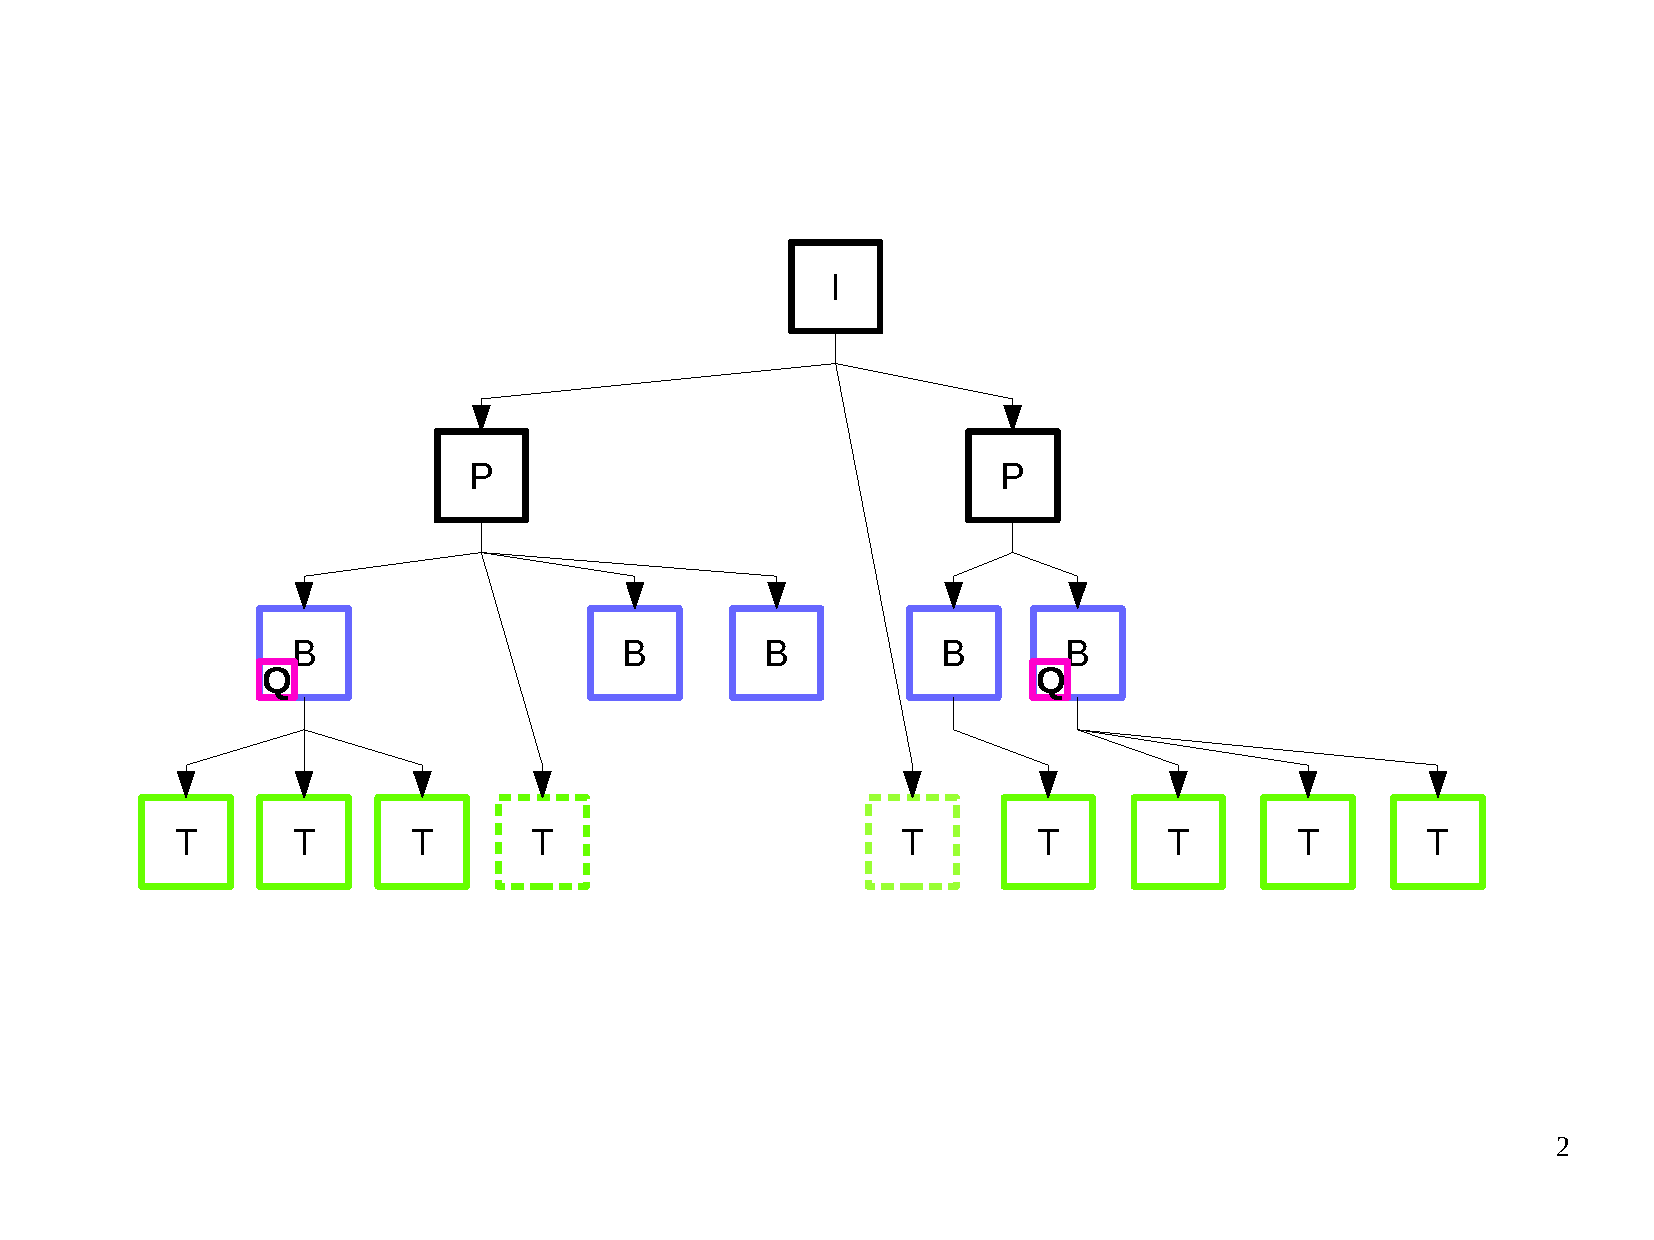
\includegraphics[trim= 65px 168px 20px 110px, clip, width=0.55\textwidth]{graph_valid_1.pdf}}
   %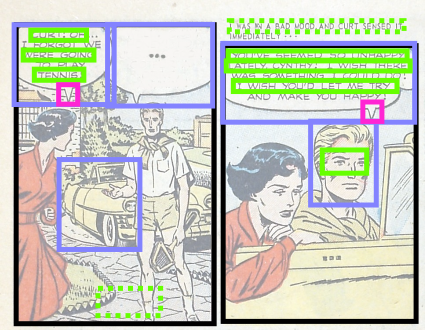
\includegraphics[trim= 0px 0px 0px 0px, clip, width=0.5\textwidth]{process_illustration_valid_1.png}\\
  %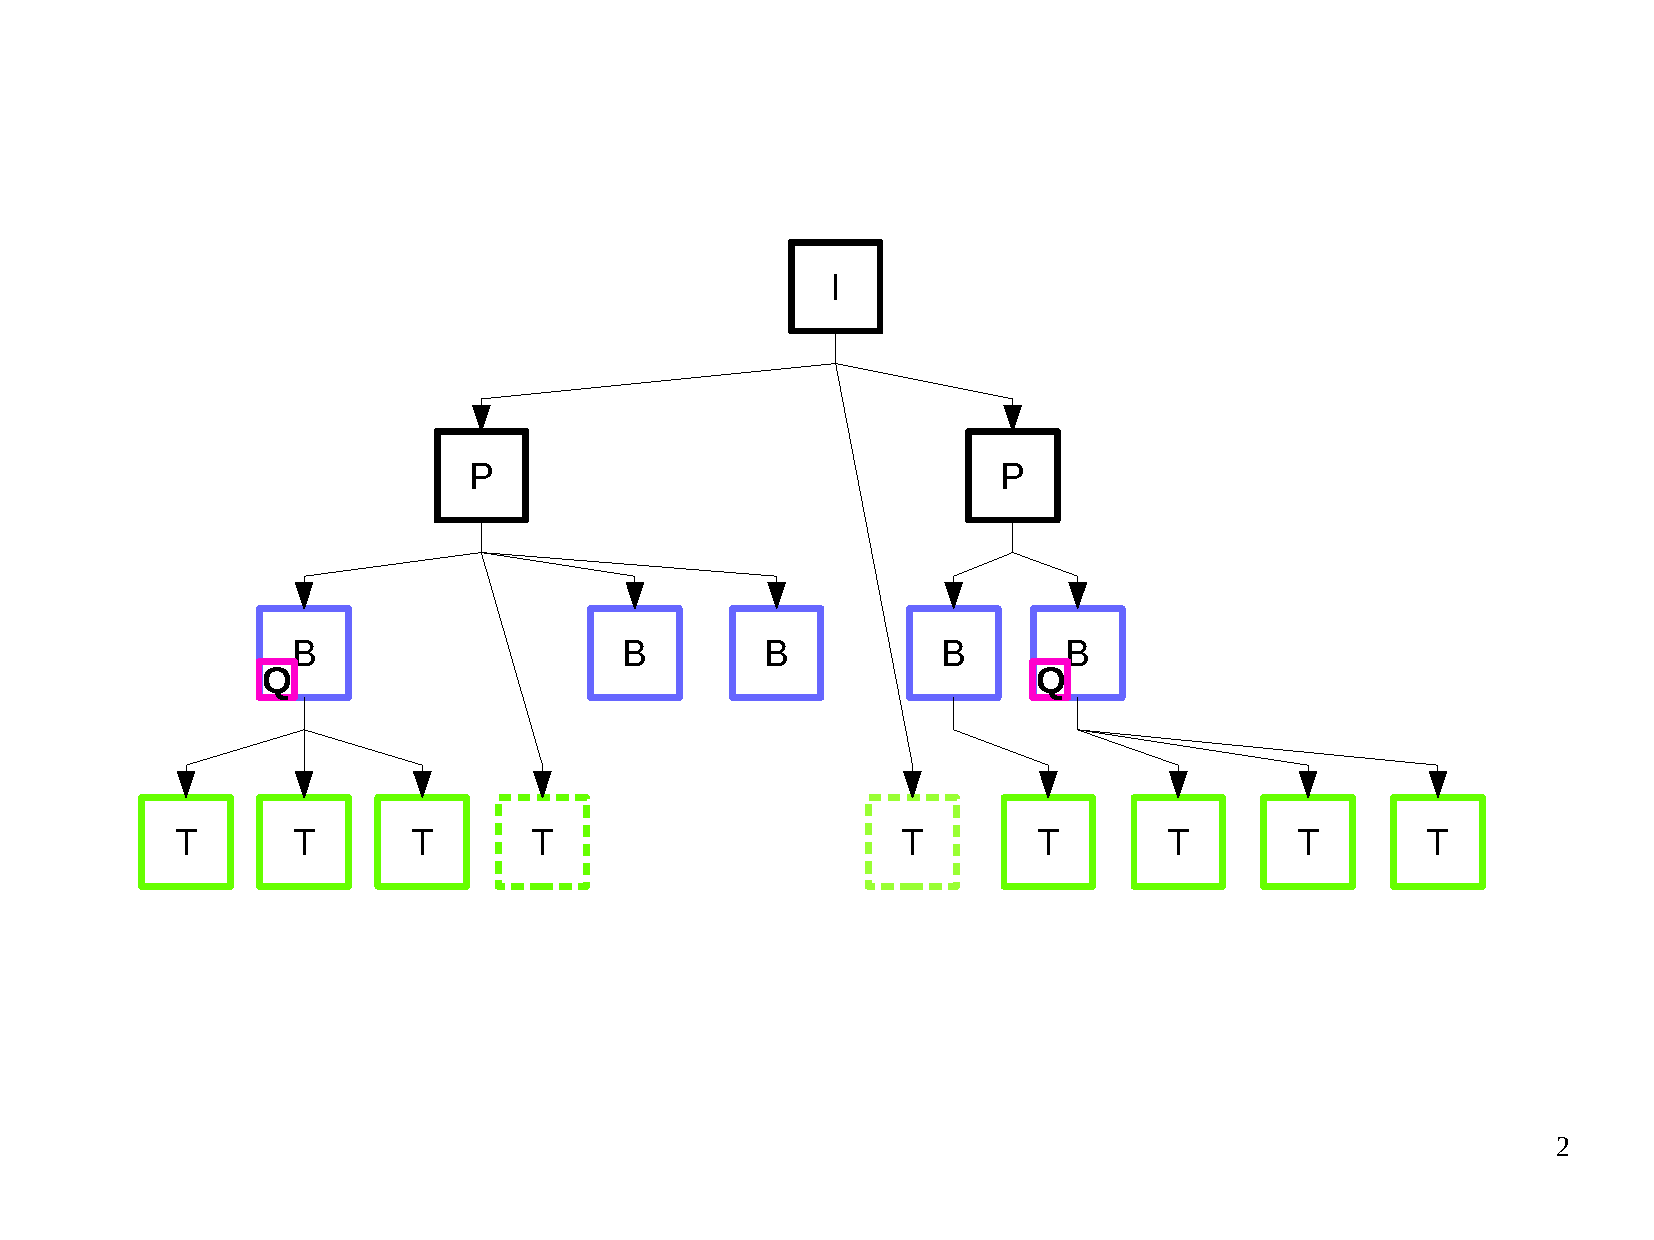
\includegraphics[trim= 30px 168px 20px 110px, clip, width=0.8\textwidth]{graph_valid_1.pdf}
  \caption[Validation of the hypothesis using the constraints of the knowledge base]{Validation of the hypothesis using the constraints of the knowledge base. Valid elements have a solid border.}
  \label{fig:kn:graph_valid_initial}
 \end{figure}
%%%%%%%%%%%%%%%%%%%%%%%%%%%%%%%%%%%%%%%%%%%%%%%%%%%

\paragraph{Iteration 1 - step 3 (inference)} % (fold)
\label{par:step_3}

At this step of the first iteration, the inconsistencies have been resolved and the remaining elements are in accordance with our model.
They are organized in the hierarchy of concepts in $\mathcal{O}_{comics}$.
The ontology being consistent, the inference engine is able to classify instances of  \concept{Balloon} and \concept{TextLine} into \concept{SpeechBalloon}, \concept{NarrativeBalloon}, \concept{SpokenTextLine} and \concept{NarratedTextLine} according to their properties and constraints.
The classification of the region instances is shown Figure~\ref{fig:kn:graph_specific_types}.
%From the validated information, the expert system infers the semantic information between text and balloon and specifies them as speech balloon and speech text respectively when they verify the properties of the knowledge base (Figure~\ref{fig:kn:graph_specific_types}). 

%%%%%%%%%%%%%%%%%%%%%%%%%%%%%%%%%%%%%%%%%%%%%%%%%%%
 \begin{figure}[!ht]  %trim=l b r t  width=0.5\textwidth,
   \centering
  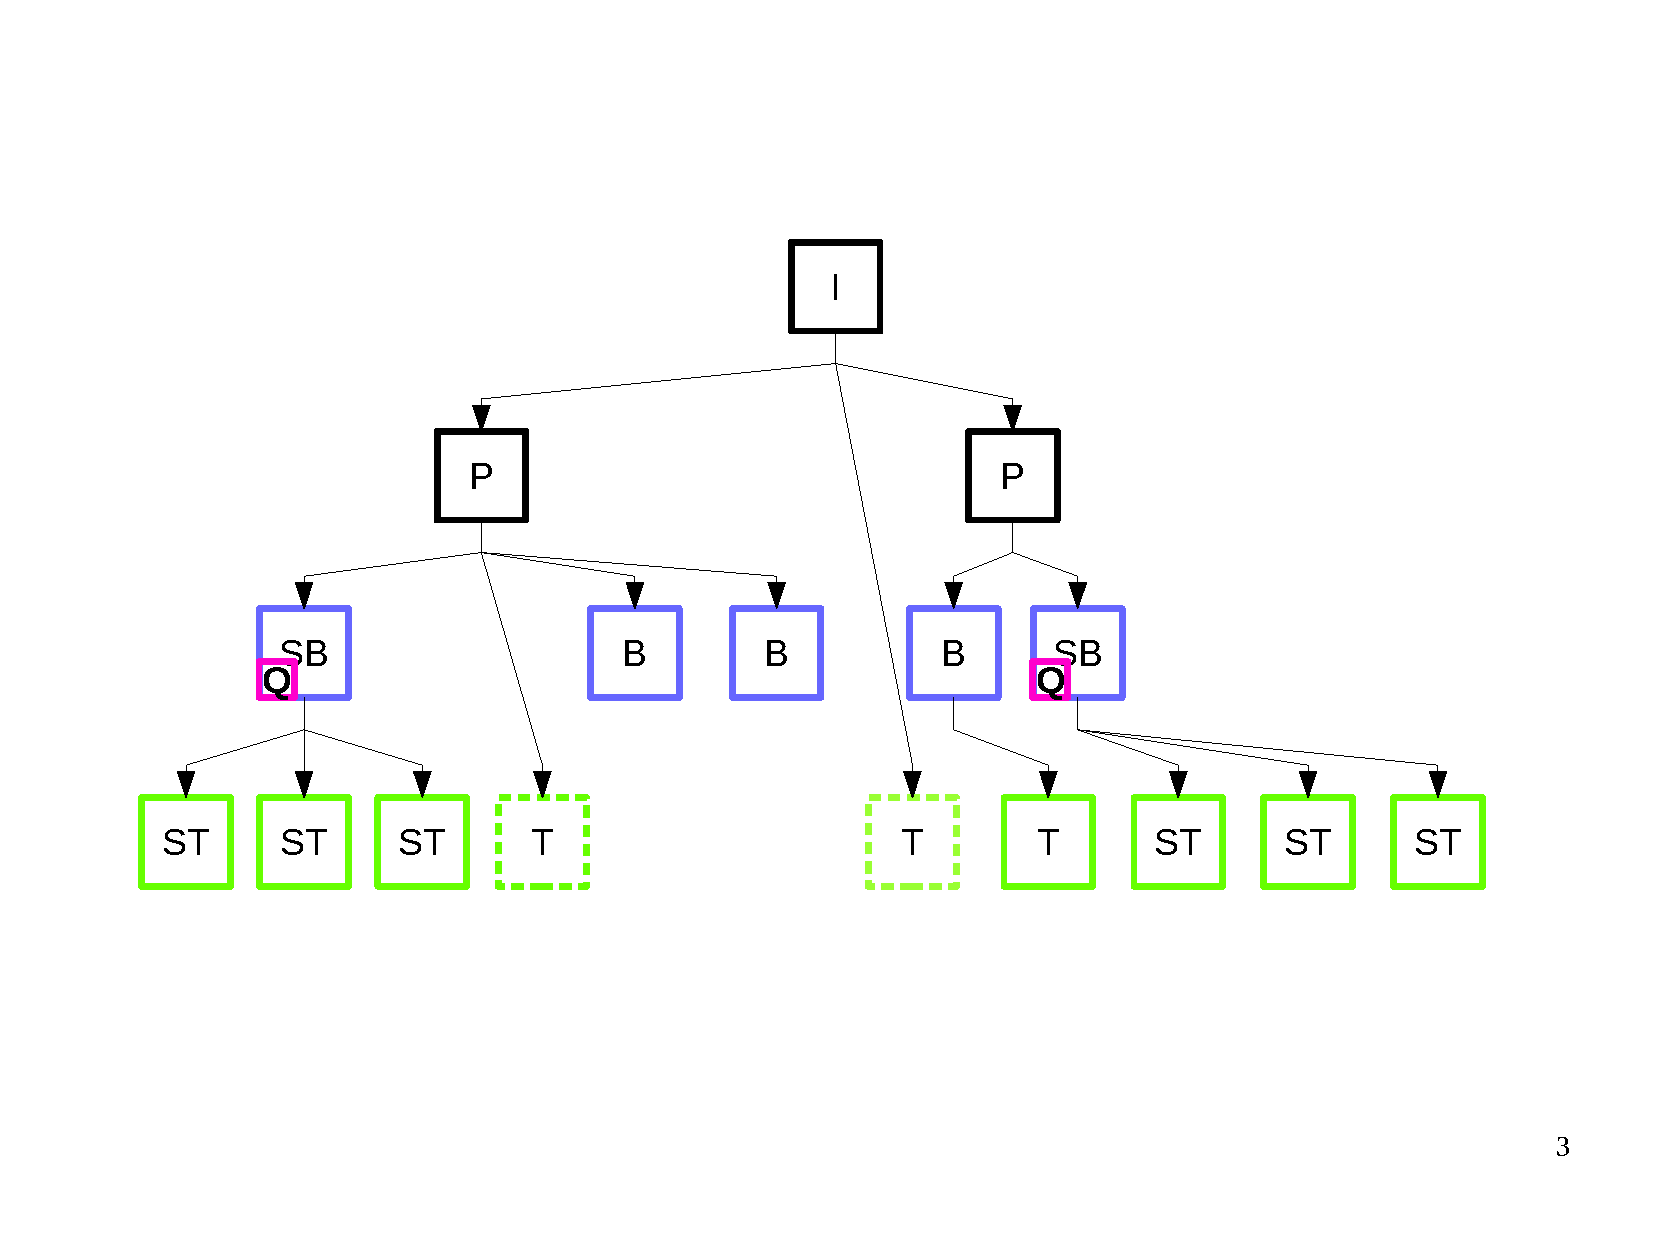
\includegraphics[trim= 30px 168px 20px 110px, clip, width=0.8\textwidth]{graph_infer_1.pdf}
  \caption[Inference of the speech balloons, narrative balloons, spoken text lines and narrated text lines using the semantic properties of the knowledge base]{Inference of the speech balloons $SB$, narrative balloons $NB$, spoken text lines $ST$ and narrated text lines $NT$ using the semantic properties and constraints of $\mathcal{O}_{comics}$.
  }
  \label{fig:kn:graph_specific_types}
 \end{figure}
%%%%%%%%%%%%%%%%%%%%%%%%%%%%%%%%%%%%%%%%%%%%%%%%%%%

% subsection simple_element_extraction (end)

\subsection{Complex element extraction} % (fold)
\label{sub:complex_element_extraction}

This is the beginning of the second iteration of the process (Figure~\ref{fig:kn:process_loop}) where we focus on more complex elements such as the comic characters.
At this point, the expert system has some information about the content of the page from the analysis carried out during the first iteration.

\paragraph{Iteration 2 - step 1 (hypothesis)} % (fold)
\label{par:step_4}

The information discovered during the first iteration of the process is used to formulate hypotheses about the probable location of the characters in the panels in order to guide their detection by the low level processing.
We first focus on characters that are emitting at least a speech balloon (considered as main characters).
It is reasonable to consider that the speech balloon and the character emitting the balloon belong to a same panel.
It is therefore possible to restrict the search space of the character inside the panel.
In addition, the position of the character in the panel can be estimated according to the direction pointed by the tail which is a characteristic of speech balloons (Figure~\ref{fig:kn:process_illustration_hypo_2_1bis}).
The estimation of the position of the comic character from the tail position and direction have been presented in Section~\ref{sec:se:tail_to_character}.
The estimated region of interest are given as seeds to the image processing algorithm (extractor of characters) which refines the regions according to the image content (Figure~\ref{fig:kn:process_illustration_hypo_2_2}).
The last step from the low level processing consists in spotting all the comic characters from the estimated examples (Figure~\ref{fig:kn:process_illustration_hypo_2_3}).

% \modif{
The method used for ROI refinement is currently under investigation and a first approach could be to fit the estimated ROI to the set of regions that are mainly overlapped by the ROI and exclude the others.
The spotting approach is relevant for retrieving non speaking characters as demonstrated Section~\ref{sec:in:character_spotting} but it is currently only appropriate for colourful comics.

%*** JCB 2014-09-16 ***
%TODO
%Tu peux dire que c'est en cours...  Mais suggérer une idéesans l'avoir testé est peut être maladroit .Soit tu dis que pour le moment tu as développé une méthode simple pour tester la partie dirigée par les modèles  comme par exemple la méthode pour les bd couleurs...  (et la prochaine étape sera pour les images N&B) Soit tu dis rien... mais ce n'est peut être pas le meilleur choix
% }

% Knowing the position of the valid from the valid triplets of panel, text and balloon.
% This is the starting point of the second iteration.

%%%%%%%%%%%%%%%%%%%%%%%%%%%%%%%%%%%%%%%%%%%%%%%%%%%
 \begin{figure}[!ht]  %trim=l b r t  width=0.5\textwidth,
   \center
  %  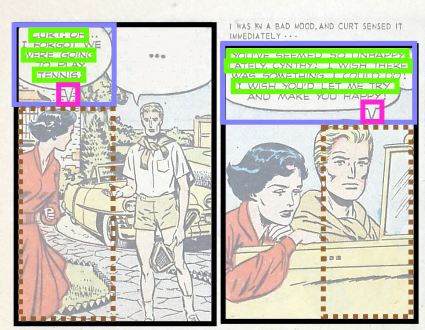
\includegraphics[trim= 0px 0px 0px 0px, clip, width=0.5\textwidth]{process_illustration_hypo_2_1.png}\\
  % 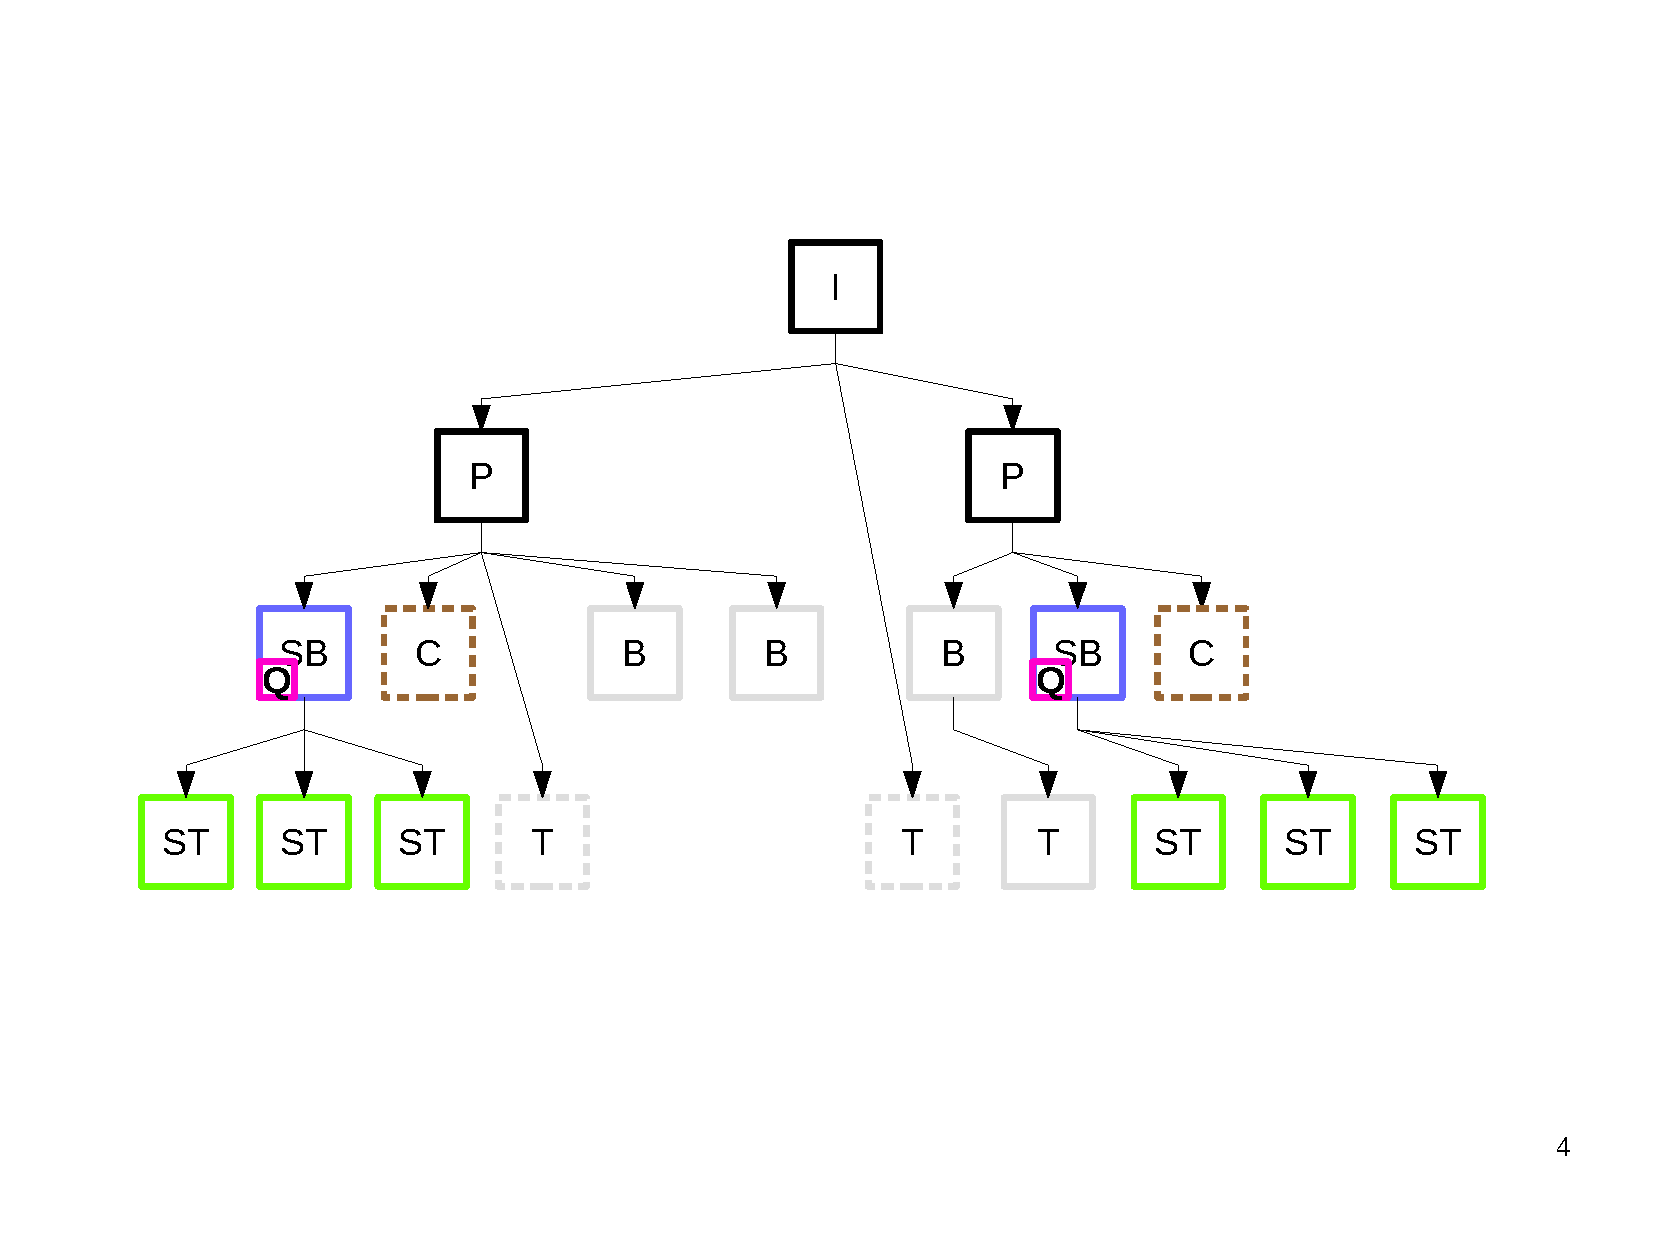
\includegraphics[trim= 30px 168px 20px 110px, clip, width=0.8\textwidth]{graph_init_2_1.pdf}
  %\subfloat[Hypothesis regions]{\label{fig:kn:process_illustration_hypo_2_1}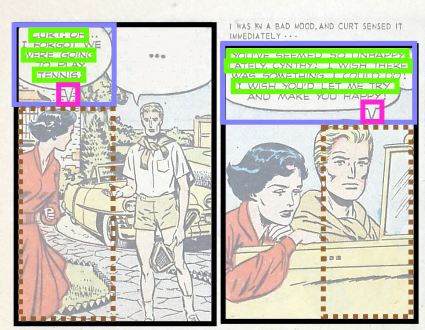
\includegraphics[width=0.45\textwidth]{process_illustration_hypo_2_1.png}} \hspace{0.5em}
   \subfloat[Hypothesis regions]{\label{fig:kn:process_illustration_hypo_2_1bis}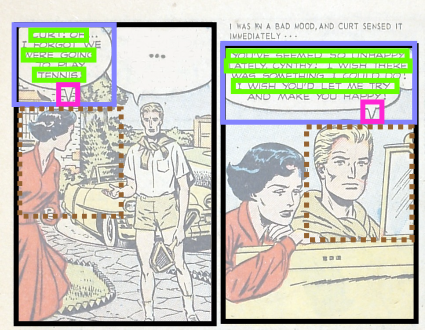
\includegraphics[trim= 0 0 0 0, clip, width=0.45\textwidth]{process_illustration_hypo_2_1bis.png}} \hspace{1em}
   \subfloat[Refined regions]{\label{fig:kn:process_illustration_hypo_2_2}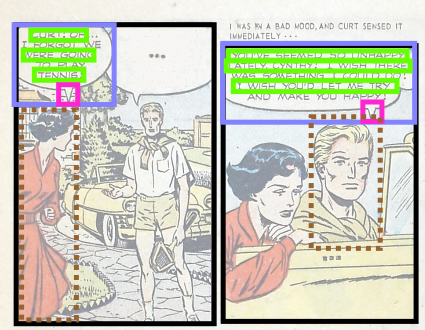
\includegraphics[trim= 0 0 0 0, clip, width=0.45\textwidth]{process_illustration_hypo_2_2.png}}\\
   \subfloat[Spotted regions]{\label{fig:kn:process_illustration_hypo_2_3}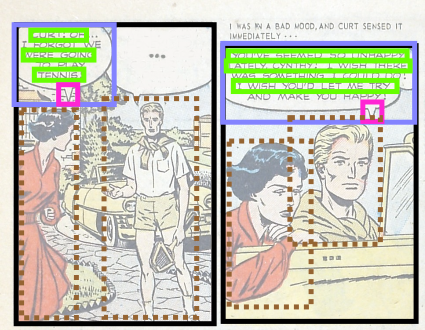
\includegraphics[trim= 0 0 0 0, clip, width=0.4\textwidth]{process_illustration_hypo_2_3.png}} \hspace{0.5em}
   \subfloat[Knowledge representation]{\label{fig:kn:graph_init_2_2}\includegraphics[trim= 65px 168px 20px 110px, clip, width=0.55\textwidth]{graph_init_2_2.pdf}}
  \caption[Hypothesis, refinement and spotting of comic character regions from the speech balloon regions]{Hypothesis, refinement and spotting of comic characters regions $C$ from the speech balloon $SB$ regions. The regions that are not related to $ST$ have been shaded in the graph and removed from the image to make it more comprehensible.
  }
  \label{fig:kn:graph_character_region}
 \end{figure}
%%%%%%%%%%%%%%%%%%%%%%%%%%%%%%%%%%%%%%%%%%%%%%%%%%%


%%%%%%%%%%%%%%%%%%%%%%%%%%%%%%%%%%%%%%%%%%%%%%%%%%%
 % \begin{figure}[!ht]  %trim=l b r t  width=0.5\textwidth,
 %   \centering
 %   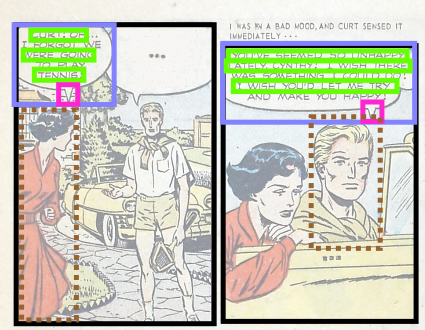
\includegraphics[trim= 0px 0px 0px 0px, clip, width=0.5\textwidth]{process_illustration_hypo_2_2.png}\\
 %  % \includegraphics[trim= 0px 168px 20px 85px, clip, width=0.8\textwidth]{fig/graph_init_2_2.pdf}
 %  \caption[Character locations $C$ returned by the low level processing]{Character locations $C$ returned by the low level processing from the ROIs defined in Figure~\ref{fig:kn:hypothesis_roi}.
 %  }% added into the graph and the corresponding region in the image $I$.}
 %  \label{fig:kn:graph_character_region}
 % \end{figure}
%%%%%%%%%%%%%%%%%%%%%%%%%%%%%%%%%%%%%%%%%%%%%%%%%%%

\paragraph{Iteration 2 - step 2 (validation)} % (fold)
\label{par:step_5}

The validation of the new regions is performed in the same way as for the first iteration.
This new batch of extraction is submitted to the constraints of the ontology as following:

\begin{itemize}
  \item \textbf{A page (p) contains a character (c)}: p is deleted.
  \item \textbf{A balloon (b) contains a character (c)}: c is deleted.
  \item \textbf{A text line (t) contains a character (c)}: c is deleted.
  \item \textbf{A character (c) contains a panel (p), a balloon (b) or a text line (t)}: c is deleted.  
  \item \textbf{A character (c1) contains a character (c2)}: c2 is deleted.
\end{itemize}
  
% The expert system checks if the spatial relations of the characters $C$ match the properties of the knowledge base defined in Section~\ref{sec:kn:constrains_low_level_extraction} 

Validated elements are represented with a solid line Figure~\ref{fig:kn:valid_2}.


%%%%%%%%%%%%%%%%%%%%%%%%%%%%%%%%%%%%%%%%%%%%%%%%%%%
 \begin{figure}[!ht]  %trim=l b r t  width=0.5\textwidth,
   \centering
  %  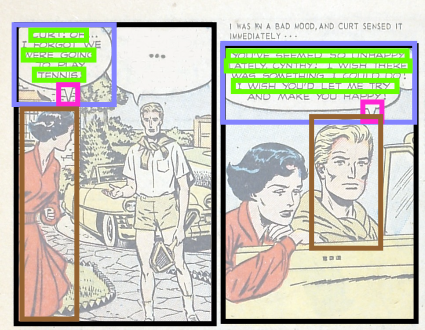
\includegraphics[trim= 0px 0px 0px 0px, clip, width=0.5\textwidth]{process_illustration_valid_2.png}\\
  % 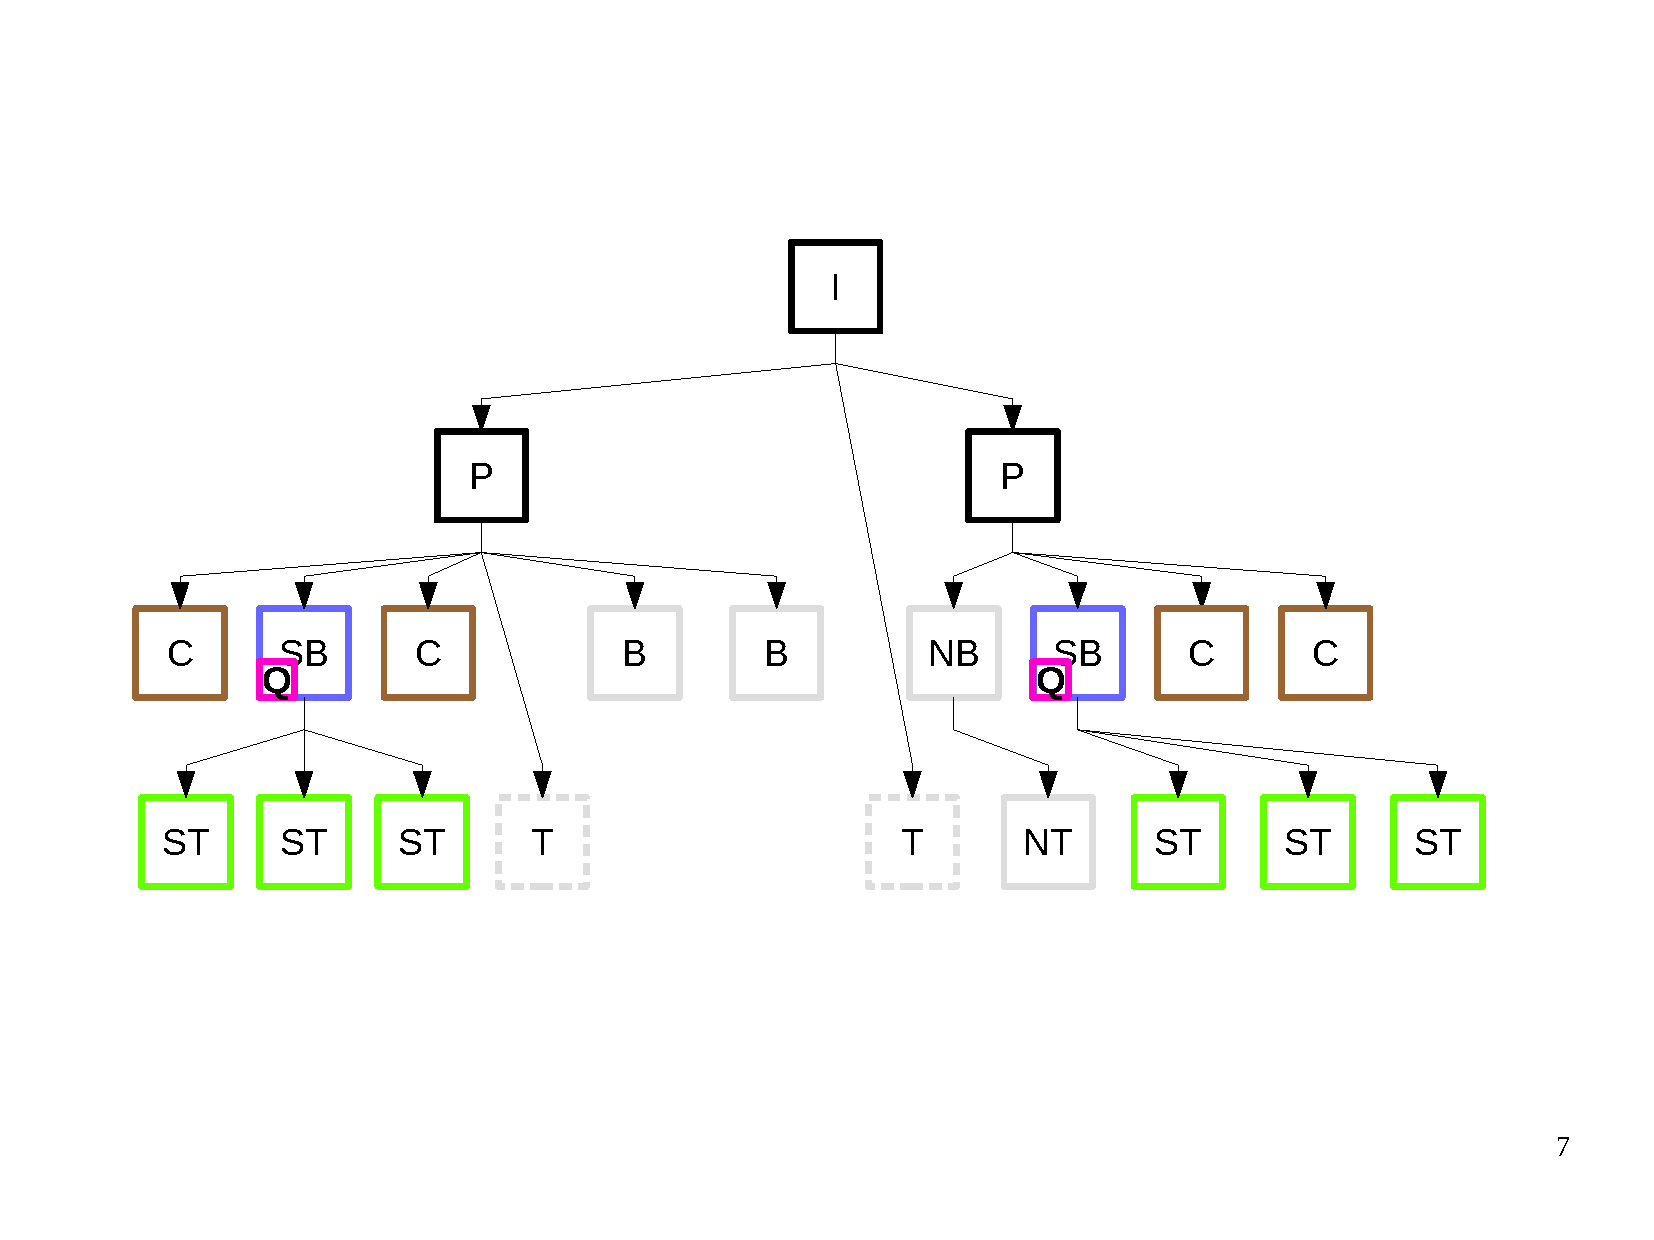
\includegraphics[trim= 0px 128px 20px 85px, clip, width=0.8\textwidth]{graph_valid_2.pdf}
  \subfloat[]{\label{fig:kn:process_illustration_valid_2}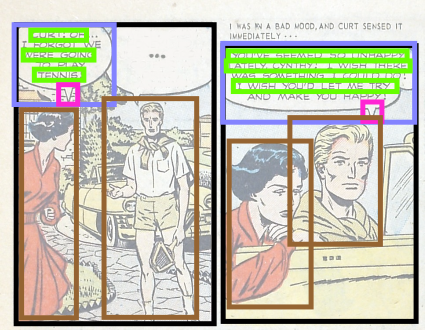
\includegraphics[width=0.4\textwidth]{process_illustration_valid_2_2.png}} \hspace{0.5em}
   \subfloat[]{\label{fig:kn:graph_valid_2}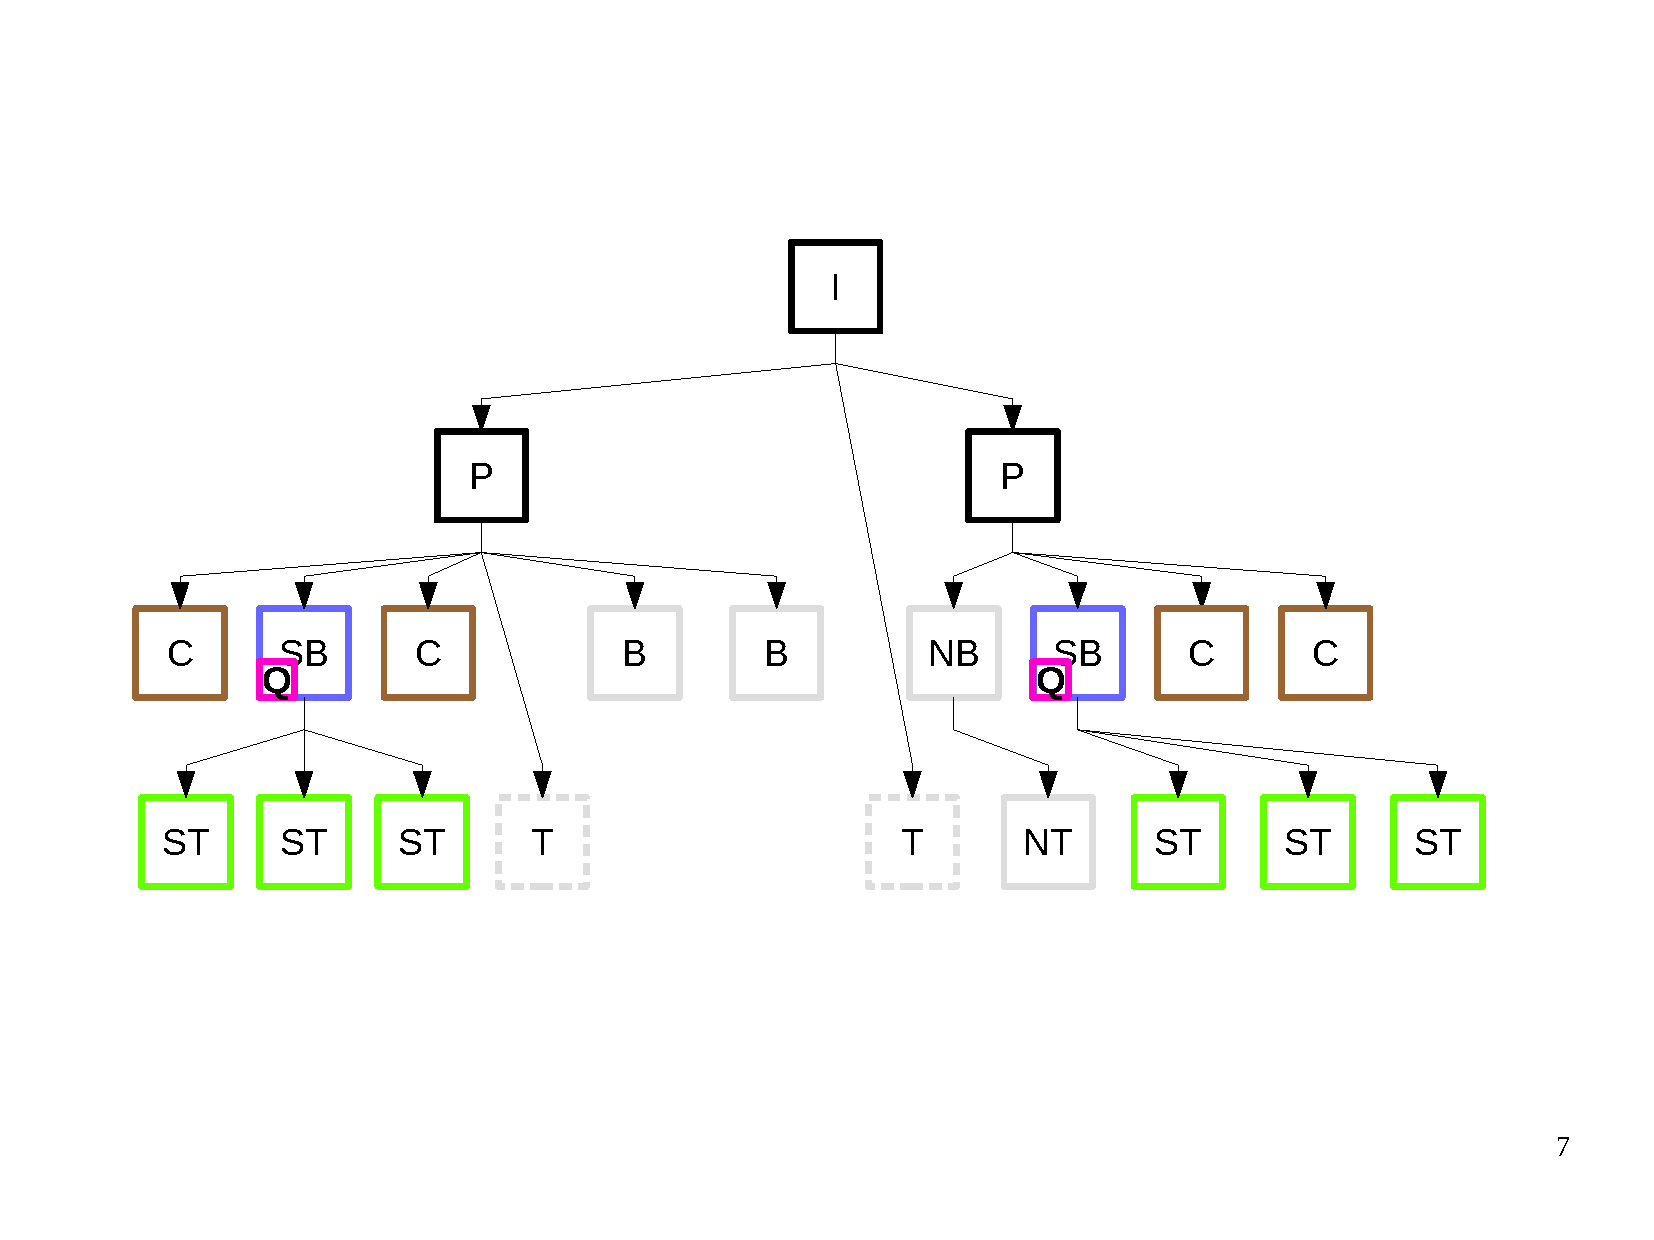
\includegraphics[trim= 65px 168px 20px 110px, clip, width=0.55\textwidth]{graph_valid_2.pdf}}
  \caption[Validation of the character regions by the expert system]{Validation of the character regions $C$ by the expert system and the corresponding image $I$.
  }
  \label{fig:kn:valid_2}
 \end{figure}
%%%%%%%%%%%%%%%%%%%%%%%%%%%%%%%%%%%%%%%%%%%%%%%%%%%

\paragraph{Iteration 2 - step 3 (inference)} % (fold)
\label{par:step_6}

The final step of this process is to deduce from all validated characters those that are actually linked to speech balloons.
Among the validated characters, we consider as being potential speakers those who intersect with the initial estimation of region of interest (Figure~\ref{fig:kn:process_illustration_hypo_2_1bis}).
An abstract straight line is drawn from each speech balloon tail tip in the direction indicated by the tail to its related panel border.
The first region of a potential speaker that it touches is considered to be the source of the speech balloon (the emitter).
This relation was asserted into the ontology with the property \textit{isSaidBy}, between the selected character and the corresponding balloon.
Since the range of this property was set to the concept of \concept{speaker}, it automatically classifies the character instance involved into this class (Figure~\ref{fig:kn:final_information}).

% The expert system infers which characters are speaking $SC$ (Section~\ref{sub:inference_of_the_speaking_characters}) and makes a semantic link to the corresponding speech balloons (Figure~\ref{fig:kn:final_information}).


%%%%%%%%%%%%%%%%%%%%%%%%%%%%%%%%%%%%%%%%%%%%%%%%%%%
 \begin{figure}[!ht]  %trim=l b r t  width=0.5\textwidth,
   \centering
  %  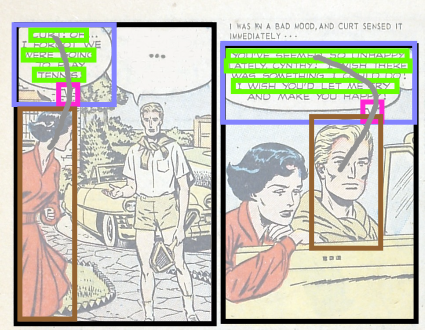
\includegraphics[trim= 0px 0px 0px 0px, clip, width=0.5\textwidth]{process_illustration_infer_2.png}\\
  % 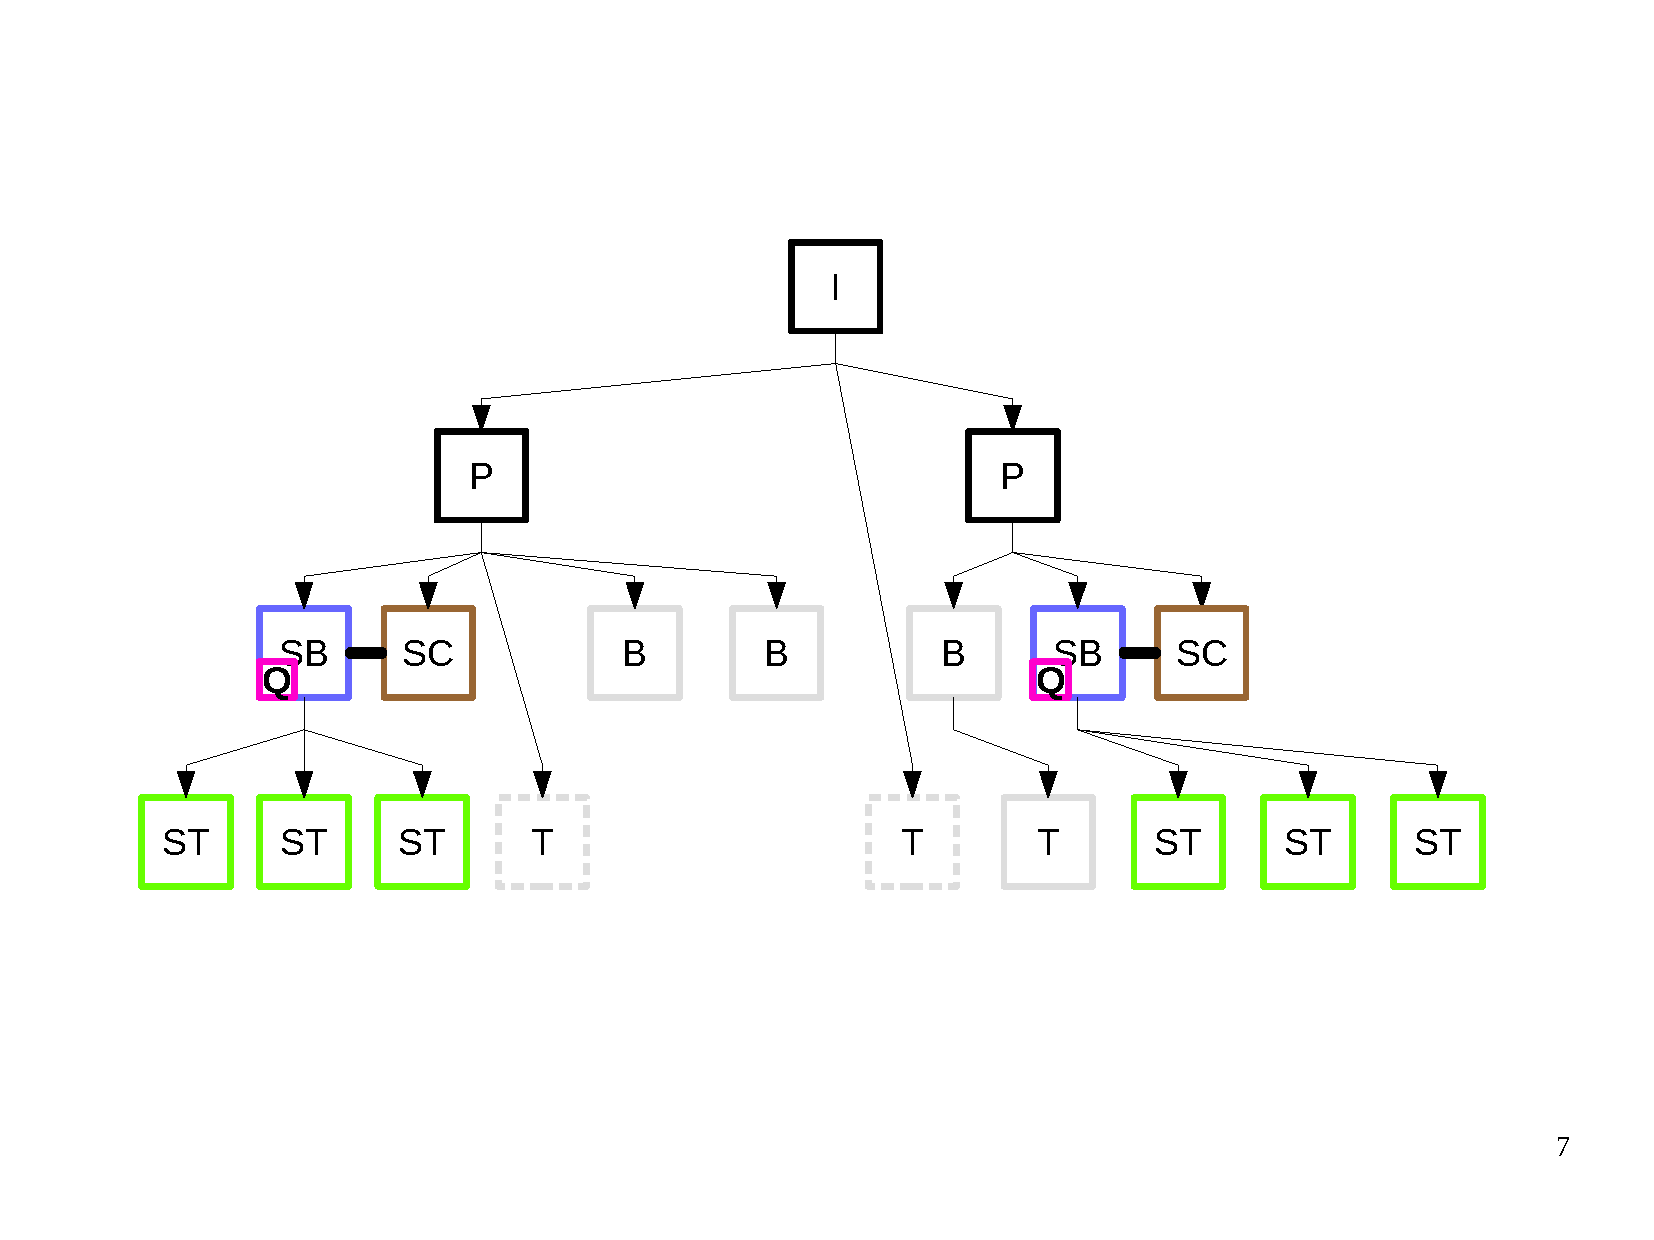
\includegraphics[trim= 0px 128px 20px 85px, clip, width=0.8\textwidth]{graph_infer_2.pdf}
  \subfloat[]{\label{fig:kn:process_illustration_infer_2}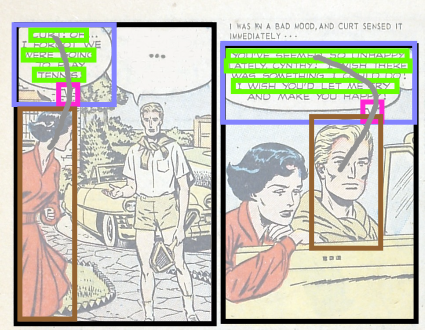
\includegraphics[width=0.4\textwidth]{process_illustration_infer_2.png}} \hspace{0.5em}
   \subfloat[]{\label{fig:kn:graph_infer_2}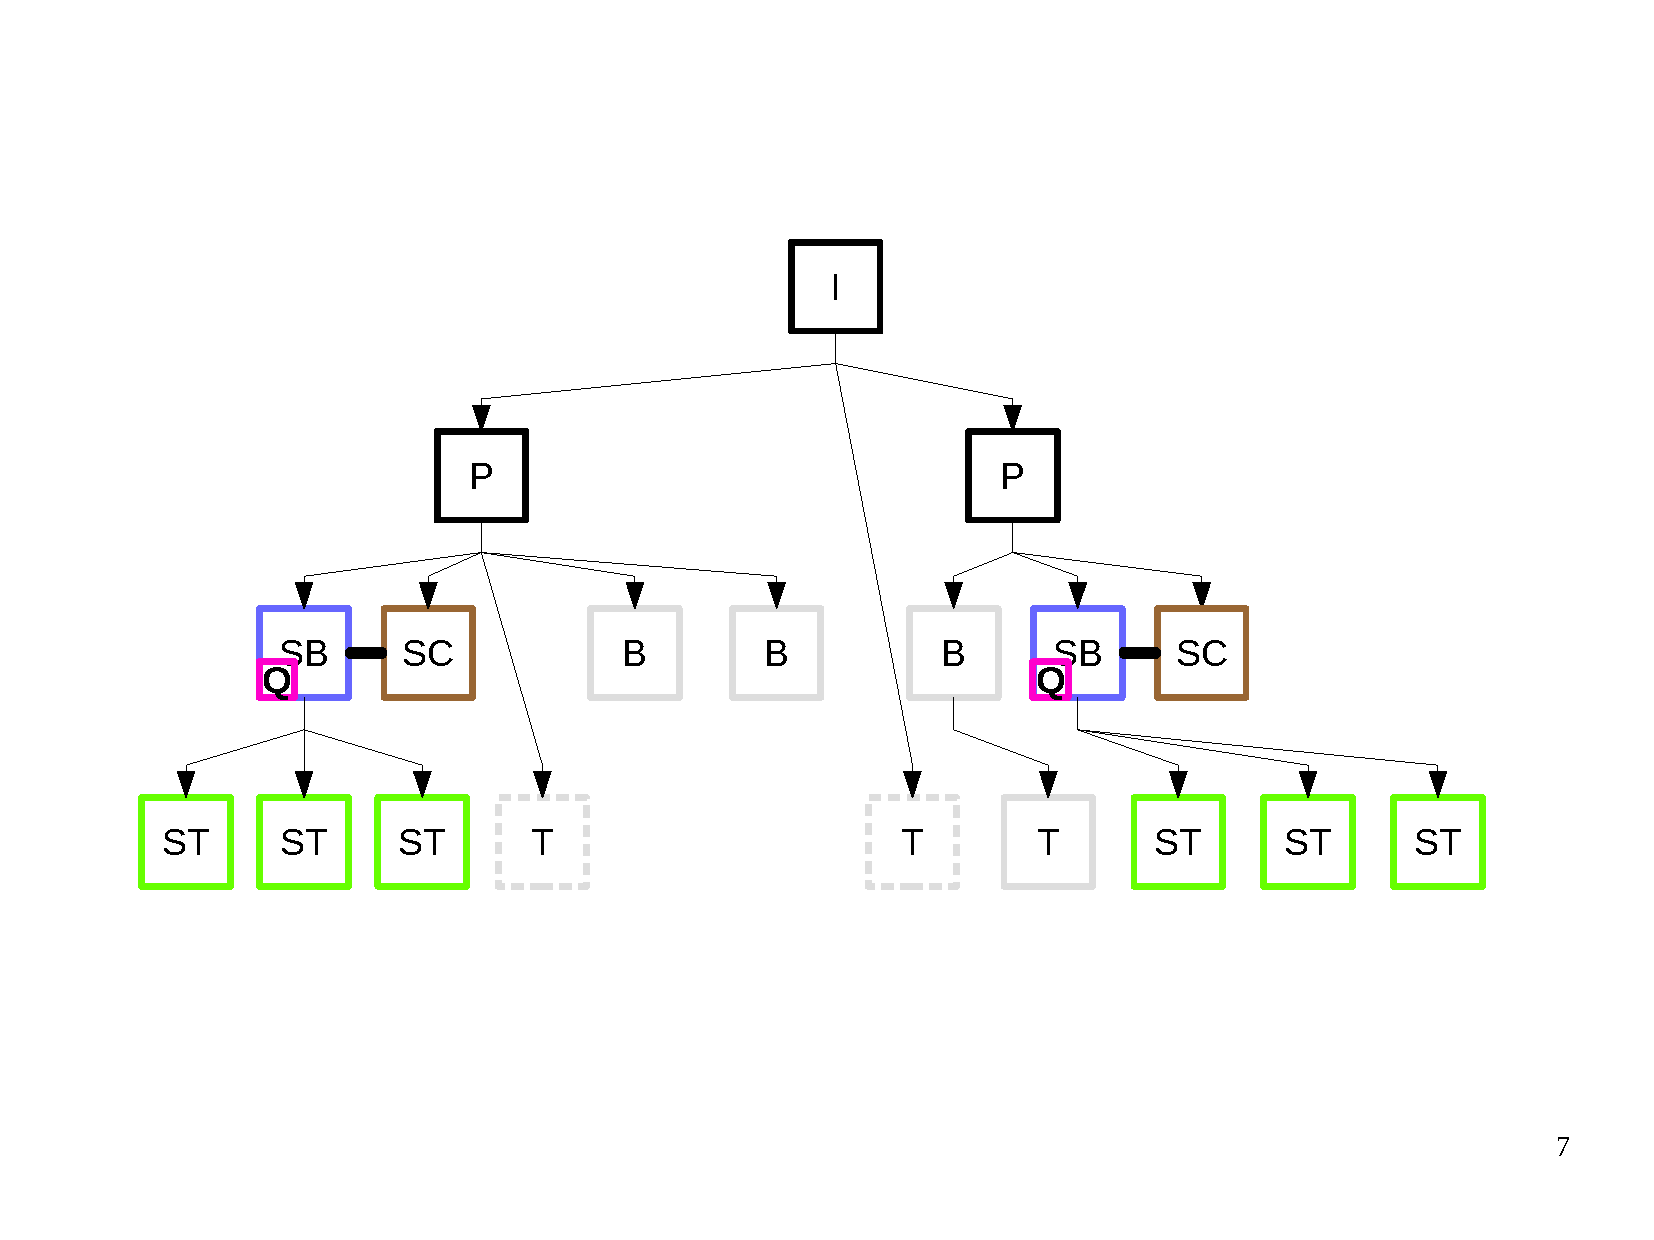
\includegraphics[trim= 65px 168px 20px 110px, clip, width=0.55\textwidth]{graph_infer_2.pdf}}
  \caption[Inference of the speaking characters and their corresponding semantic links to speech balloons]{Inference of the two speaking characters $SC$ and their corresponding semantic links to speech balloons $SB$ regions.
  The two semantic links are represented by a grey stroke in the image over the regions concerned and a non-oriented horizontal edge in the graph.
  }
  \label{fig:kn:final_information}
 \end{figure}
%%%%%%%%%%%%%%%%%%%%%%%%%%%%%%%%%%%%%%%%%%%%%%%%%%%

At the end of the two iterations we obtained both a topological and a semantic description of the image content, illustrated in a single graph here.
Further iteration could be processed by extracting other low level elements such as faces or vehicles and by adding extra domain knowledge.


% subsection complex_element_extraction (end)

% section framework_ (end)

% \section{Presentation of the models} % (fold)
% \label{sec:kn:model}

% The knowledge base is composed of two ontologies, designed using OWL's W3C recommendation~\cite{McGuinness2004}, and interacting with each other (Figure~\ref{fig:kn:generic_expert_system}).
% The first one was used to model the raw data provided by image analysis algorithms (called \textit{image model} hereafter), while the second models the comic book domain knowledge (called \textit{comics model}).
% These two models are bounded by bridges that are used to perform reasoning over both models, using their own properties.

% \subsection{Image model}


% \subsection{Comics model}


% \subsection{Model interactions}
% The image and comics models are linked through two bridges.
% First, the \textit{Image} from the image model and \textit{Page} from the comics model concepts are made equivalent by the axiom \texttt{owl:equivalentClass}.
% This way we ensure that all extracted content related to an image is equally related to a corresponding page in the comics domain $Page \equiv  Image$.

% Second, the classes $Cl=\{Panel$, $Balloon$, $TextLine$, $Character\}$ are defined as equivalent to the corresponding set of regions of interest $Sr = \{panels$, $balloons$, $text lines$, $characters\}$ Equation~\ref{eq:kn:class_region_equivalence}).% that have an extractor which purpose is to extract the corresponding panels (resp. balloons, text lines and characters).
	

% \begin{equation}
% \label{eq:kn:class_region_equivalence}
% \begin{split}
% Cl_i  \equiv \text{ROI} \textbf{ and } (hasExtractor \textbf{ some } (roiType \textbf{ value } Sr_i ))
% \end{split}
% \end{equation}

% section model (end)

% \modif{

% \section{Interactions between high and low level processing}
% \label{sec:kn:interaction_low_high_level_processing}

% \modif{TODO: to dispatch in processing sequence subsection}

%This section describes how the extracted data are processed at the semantic level.
% This section presents the low and high level processing interaction to validate the extractions, infer information and generate hypotheses about the image content.% we use it to validate the extracted elements, infer more information about them and express region of interest's hypothesis to send back at low-level algorithms.
% \subsection{Validation of the extractions} % (fold)
% \label{sub:kn:validation}
% In order to validate the extraction of the comic page's components, we made sure that the extracted panels, balloons and text lines were in accordance with the knowledge defined in \ref{sec:kn:constrains_low_level_extraction}.
% %Those which are not consistent with our model are rejected.

% Firstly, each item was loaded into the model as it was labelled (page, panel, balloon, text line or comics character) by the low level processing step.
% Then, each element was linked to its smallest container in a half-blind way (Section~\ref{sec:kn:constrains_low_level_extraction}).
% That is to say that the type of contained element was known, while the type of  potential container was not.
% Not knowing the type of container might have lead to incorrect assertions that would have produced inconsistencies in the model.
% Those inconsistencies are the result of possible mistakes made during the extraction process that were filtered out in order to improve the overall detection precision.
% Consistency checking was performed over the model and inconsistencies were handled one after the other.
% We chose to focus on increasing the extraction precision by deleting those elements that did not fit the constrained model.
% The detection of misclassified elements (a panel actually being a balloon) and the proposition of missed elements (like a missed balloon around a group of text lines) were both perspectives of this work.
% For the time being, our system can handled, without being limited to, the following inconsistencies:
% %Due to the limited number of object types we deal with, inconsistencies sources can be reduced to this exhaustive list:

% \subsection{Inferences from the low level information} % (fold)
% \label{sub:inference_from_low_level}

% The expert system is able to infer more specific information than that given by the extractors.
% For instance, it can deduce which text is spoken or not and which speaking character pronounces the content of which speech balloon.

% % Use of RDFS/OWL (Web ontology language) to model the information domain with the general comics properties listed bellow, base on the type of region given by the low level processing:

% % subsection inference_ (end)

% % \subsection{Region of interest of character (step 4)} % (fold)
% % \label{sub:speaking_region}
% % TO COMPLETE (Clement?)

% The expert system infers the speaking character location from valid speech balloons regions by computing a region from the tail tip to the panel side following the tail direction, for each speech balloon.
% ...
% Those regions are voluntary quite large to maximize the chance to cover at least the speaking characters.

% The regions are passed to the image processing part (character extractor) that will extract all the characters using those regions as seeds.

% \paragraph{Speech balloon and speech text} % (fold)
% \label{par:speech_balloon_and_speech_text}

% The classification of balloons and text respectively into speech balloons and spoken text can be done by running an inference engine on the model (e.g. Racer~\cite{Haarslev2012}] or Pellet~\cite{Sirin2007a}).
% To allow reasoning, the model has to be consistent, which is the case after validation step~\ref{sub:kn:validation} when all inconsistencies have been resolved.
% In Section~\ref{sec:kn:constrains_low_level_extraction}, we defined a speech balloon as a balloon that has a tail.
% In others words, the concept of a \textit{speech balloon} can be seen as a specialization of the \textit{balloon} concept that extends all its properties plus adding a few new ones.
% This is expressed in the expert system by defining a property \textit{hasTail} with the constraint that must have a \textit{speech balloon} instance as a source.
% Assessing this piece of knowledge, the reasoner will automatically deduce that each instance of \textit{balloon} extended with a \textit{hasTail} property can be specialized into a \textit{speech balloon}.

% In a similar way, the concept of \textit{text line} subsumes the concept of \textit{spoken text line}.
% It is rendered equivalent to the set of individuals from the \textit{text line} concept that is bound with the property \textit{isLineOf}, which is the inverse property of \textit{hasLine}, to a \textit{speech balloon}.
% In other words, the text lines marked as being part of a speech balloon are automatically classified as spoken text lines.


% \paragraph{Speaking characters} % (fold)
% \label{sub:inference_of_the_speaking_characters}

% Among the validated characters (Section~\ref{sub:kn:validation}), we considered as being potential speakers those who intersect with the hypothetical region computed in \ref{sec:se:tail_to_character}.
% These regions were computed from each speech balloon, i.e. the balloons that had an identified tail.
% An abstract straight line was drawn from that tail tip in the direction indicated by the tail.
% The first region of a potential speaker that it touched was considered to be the source of the speech balloon.
% This relation was asserted into the ontology with the property \textit{isSaidBy}, between the selected character and the corresponding balloon.
% Since the range of this property was set to the concept of \textit{speaking character}, it automatically classified the character instance involved into this class.

% section interaction_low_high_level_processing (end)

% \subsection{Hypothesis} % (fold)
% \label{sub:hypothesis}

% \modif{TODO: ROI same as Method 1, reading order (7.2 Clement), other from Clement's thesis (coming soon)}

% subsection hypothesis (end)

% Conclusion --------------------------------------------------------------------------------------------------------------------------------------
\section{Conclusions}
\label{sec:kn:conclusion}

We presented a new framework for understanding documents that can interact with low and high level information suitable for semi structured and complex background documents such as comics.
Several key improvements to information extraction and processing methods have been developed. 

Two ontologies have been presented in this chapter, the first one is formalizing the concepts implemented for image analysis and the second one for formalizing the comics domain.
The image processing ontology has the advantage of being completely independent of any application.
The proposed comics ontology is composed of concepts that reflect the classic structure of a comic book.
This conceptualization has been developed with the target of image analysis interfacing the image ontology through equivalence relations between some of their concepts.

The proposed system provides a novel generic and unsupervised approach for comic book document understanding mixing visual and semantic information.
It relies on an inference engine that interacts with the two proposed models.
We detailed a use case for comic character localisation associated with their corresponding speech balloons, taking into account the spatial organisation of the rest of the elements in an image.
One limitation of the proposed system is the validation process which only suppresses elements until having a consistent representation of the knowledge.
We are currently working on different scenarios able to compute a cost, in terms of number of inconsistencies that are created or solved, of changing the class from one type to another one (e.g. changing a region given by the panel extractor as balloon and \emph{vice versa}).
This solution will permit to apply the changes that have the minimal cost, including deletion as the last option, in order to make the knowledge representation consistent while minimizing the loss of extracted information.

In the future we plan to add more iterations of the process in order to retrieve new information such as other objects in the panels and sound effects.
In addition, the expert system will be used to improve text extraction and recognition using system feedback in order to automatically extract open speech balloons from validated text locations.
A semantic tag (e.g. speech, thought, exclamation) can also be given to the speech text regions according to a deeper analysis of the type of balloon presented Section~\ref{sub:in:balloon_classification}.

In the next chapter, we are going to experiment the different contributions presented in this thesis and compare them to other methods from the literature.
The dataset is first introduced along with the metrics we used to evaluate information retrieval. 
